\section*{三、多面体和旋转体的体积}

对我们来说，体积并不全是新知识. 在小学里，已经学
过某些多面体和旋转体的体积公式. 例如：
\[\begin{split}
 V_{\text{长方体}}=abh=Sh,&\qquad V_{\text{正方体}}=a^3;\\
 V_{\text{圆柱}}=Sh^3,&\qquad V_{\text{圆锥}}=\frac{1}{3}Sh.   
\end{split}\]

（上式中$V$表示体积，$S$表示底面积，$h$表示高，$a$、$b$表示棱长）

在这一单元，我们要学习所有柱体、锥体、台体和球的体积公式，同时还要论证为什么应该是这样的公式. 在小学，只能采取实验的方法，粗略地给以说明. 现在我们将应用逻辑推理的方法来处理每一个公式，这就要首先提出体积的概念和一些公理作为推理的基础.

\section{体积的概念和公理}
我们知道，每一个几何体都占有一定的空间. 几何体占有空间部分的大小叫做它的\textbf{体积}.

要度量一个几何体的体积的大小，首先要选取一个单位体积作为度量的标准（这正象度量长度、面积时需要选取单位长度和单位面积一样）.度量体积时，通常取棱长等于单位长度（1cm，1m等）的正方体的体积作为体积单位．

有了体积单位后，就可求出几何体的体积是单位体积的多少倍，这个倍数就是这个几何体体积的数值（或量数），这个数值连同体积单位一起刻画了这个“几何体所占空间部分的大小”，即它的体积.

如果一个几何体恰好能分成若干个单位正方体，那么我们就容易求得这个几何体的体积，如果某些几何体不能分成若干个正方体，例如棱锥和旋转体，我们怎样计算它们的体积呢？

我们在度量体积时，以下述两个基本性质为依据：
\begin{enumerate}[(1)]
 \item 两个全等的几何体，它们的体积相等．
\item 一个几何体的体积，等于它的各部分体积的和．
\end{enumerate}

例如：把棱长等于单位长（1cm）的正方体的一个顶点作为棱锥的顶点，这个点所对的正方体的侧面或底面作为棱锥的底面，这样可将正方体分割成三个全等的四棱锥，由基本性质可知，每一个四棱锥都是$\frac{1}{3}$个单位体积，即为$\frac{1}{3}{\rm cm^3}$. 

\begin{figure}[htp]
    \centering
\begin{tikzpicture}
\begin{scope}
\tkzDefPoints{0/0/A, 2/0/B, 2.5/.7/C, .5/.7/D, 0/2/A'}
\foreach \x in {B,C,D}
{
    \tkzDefPointBy[translation = from A to A'](\x)
    \tkzGetPoint{\x'}
}
\tkzDrawSegments[dashed](A,D C,D D,D')
\tkzDrawSegments[very thick](B,B' B',A' B',C')
\tkzDrawPolygon[very thick](A,B,C,C',D',A')


\end{scope}
\begin{scope}[xshift=4cm]
    \tkzDefPoints{0/0/A, 2/0/B, 2.5/.7/C, .5/.7/D, 0/2/A'}
\foreach \x in {B,C,D}
{
    \tkzDefPointBy[translation = from A to A'](\x)
    \tkzGetPoint{\x'}
}
\tkzDrawSegments[dashed](A,D C,D D,D')
\tkzDrawSegments[very thick](B,A' B,C' B,D')
\tkzDrawPolygon[very thick](A,B,C,C',D',A')
\end{scope}
\begin{scope}[xshift=8cm]
    \tkzDefPoints{0/0/A, 2/0/B, 2.5/.7/C, .5/.7/D, 0/2/A'}
\foreach \x in {B,C,D}
{
    \tkzDefPointBy[translation = from A to A'](\x)
    \tkzGetPoint{\x'}
}
\tkzDrawSegments[dashed](B,D')
\tkzDrawSegments[very thick](B,B' B',A' B',C')
\tkzDrawPolygon[very thick](B,C',D',A')
\end{scope}
\end{tikzpicture}
    \caption{}
\end{figure}

从这个例子可知，虽然我们还不知道棱锥的体积公式，但用这两条基本性质我们却求出了正方体被分成三个全等的四棱锥时每一个棱锥的体积.

但这种情况总是少数，为了推算体积的公式，我们引入两个公理.

\begin{thm}
    {公理5} 长方体的体积等于它的长、宽、高的积．
\[V_{\text{长方体}}=abc\]
其中，$a$、$b$、$c$分别是长方体的长、宽、高.
\end{thm}

\begin{thm}
{推论1} 长方体的体积等于它的底面积$S$和高$h$的积．
\[V_{\text{长方体}}=Sh\]
\end{thm}

\begin{thm}
{推论2} 正方体的体积等于它的棱长$a$的立方．
\[V_{\text{正方体}}=a^3\]
\end{thm}

\begin{thm}
{公理6} 夹在两个平行平面间的两个几何体，被平行于这两个平面的任意平面所截，如果截得的两个截面的面积总相等，那么这两个几何体的体积相等.
\end{thm}

图2.84表示，夹在平行平面$\alpha$、$\beta$之间的两个形状不同的几何体，被平行于平面$\alpha$、$\beta$的任意一个平面所截，如果截面$P$和$Q$的面积总相等，那么它们的体积一定相等.

\noindent
\begin{minipage}{.45\textwidth}
\centering
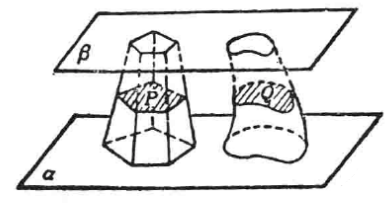
\includegraphics[scale=.45]{fig/2-84.png}
\captionof{figure}{}    
\end{minipage}
\hfill
\begin{minipage}{.53\textwidth}
    \centering
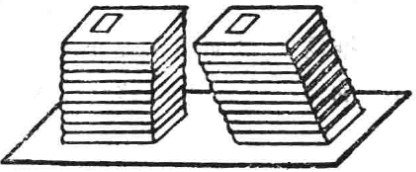
\includegraphics[scale=.45]{fig/2-85.png}
\captionof{figure}{}    
\end{minipage}


例如，取一摞书或一摞纸张堆放在桌面上，将它如图2.85那样改变一下形状，这时高度没有改变，每页纸的面积也
没有改变，因而这摞书或纸张的体积与变形前相等.

公理6是我国古代数学家祖暅\footnote{祖暅，是祖冲之的儿子，他的活动时期大约在公元504—526年，在数学和天文学上都有杰出贡献.}提出的，他指出：“缘幂势既同，则积不容异”．“幂”指的就是图2.84中的截面面$P$和$Q$．“势”指的是高$h$，也就是图2.84中的两平行平面间的
距离. 公元前五世纪时，祖暅首先使用这个原理解决了刘徽等数学家未曾解决的球体积公式推导中的关键问题，得出球体积的算法. 为了纪念他的伟大贡献我们把它叫做祖暅原理. 而在欧洲，直到1000多年以后，在17世纪，才有意大利的卡发雷利提出这个事实.

祖暅原理也可以用平面几何的事实类比推想出来.

现在把等底等高的两个三角形像图2.86那样夹在两平行线$a$、$b$之间，这时，被平行于$a$、$b$的任意一条直线所截，则截得的两条线段$DE$和$D'E'$ 总是相等的. 从而这两个三角形的面积相等. 事实上，由于 $AD:DC=A'D':D'C'$, 所以有
\[
\frac{ED}{BC}=\frac{AD}{AC}=\frac{A'D'}{A'C'}=\frac{E'D'}{B'C'}\]

\begin{figure}[htp]
    \centering
\begin{tikzpicture}
\tkzDefPoints{-3/-1/b, 3/-1/b', -3/1.5/a, 3/1.5/a', -3/.5/c, 3/.5/c'}
\tkzDrawSegments[very thick](b,b' a,a')
\tkzDefPoints[]{-2/1.5/A, 2.5/1.5/A', -2.25/-1/B, -1/-1/C, 1.25/-1/C', 0/-1/B'}
\tkzDrawSegments[very thick](A,B A,C A',B' A',C')
\tkzLabelPoints[below](B,C,B',C')
\tkzLabelPoints[above](A,A')
\tkzLabelPoints[left](a,b)
\tkzInterLL(A,B)(c,c') \tkzGetPoint{E}
\tkzInterLL(A,C)(c,c') \tkzGetPoint{D}
\tkzInterLL(A',B')(c,c') \tkzGetPoint{E'}
\tkzInterLL(A',C')(c,c') \tkzGetPoint{D'}
\tkzDrawSegments[very thick](c,D E',c')
\tkzDrawSegments[thick, dashed](D,E')
\tkzLabelPoints[above left](E)
\tkzLabelPoints[above right](D,D')
\tkzLabelPoints[above](E')

\end{tikzpicture}
    \caption{}
\end{figure}



又因$BC=B'C'$, 故$CD=C'D'$.

由公理6可以得到下面的推论：

\begin{thm}{推论1}
底面积相等并且高也相等的两个柱体（棱柱、圆柱）的体积相等. 如图2.87.
\end{thm}

\begin{figure}[htp]
    \centering
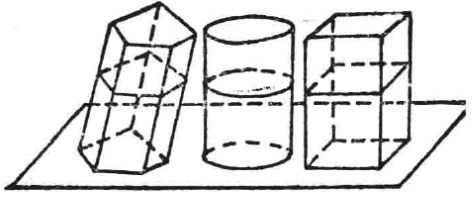
\includegraphics[scale=.5]{fig/2-87.png}
    \caption{}
\end{figure}

\begin{thm}
{推论2} 底面积相等并且高也相等的两个锥体（棱锥、圆锥）的体积相等. 如图2.88.    
\end{thm}
\begin{figure}[htp]
    \centering
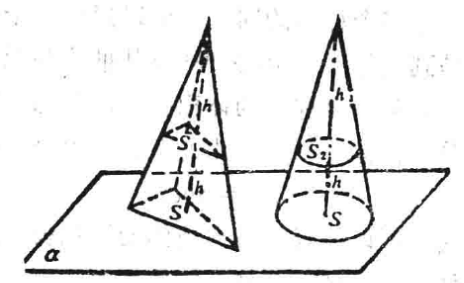
\includegraphics[scale=.5]{fig/2-88.png}
    \caption{}
\end{figure}

以上两个推论由读者自己证明.


\subsection*{2.7 练习}
\begin{enumerate}
    \item 把夹在两条平行线间的两个平面图形的面积相等的条
件，用祖暅原理的形式叙述出来. 并根据矩形面积公式$S=ab$，求平行四边形的面积公式.
\begin{figure}[htp]
    \centering
\begin{tikzpicture}[scale=1.5]
\tkzDefPoints{-2/0/a, 2/0/a', -2/2/b, 2/2/b'}
\tkzDefPoints{-1.5/0/A, 0/0/B, .2/0/C, 1.7/0/D}
\tkzDefPoints{-1/2/A', -.3/2/B', .5/2/C', 1.2/2/D'}
\tkzDrawSegments[very thick](A,A' B,B' a,a' b,b')
\draw(C)[bend right=20, thick] to (C');
\draw(D)[bend right=10, thick] to(D');
\tkzLabelPoints[left](a,b)
\draw[ thick](-1.12,1.5)--+(.9,0);
\draw[ thick](.55,1.5)--+(.85,0);
\draw[ thick](-1.26,1)--+(1.1,0);
\draw[ thick](.55,1)--+(1,0);
\draw[ thick](-1.26,.96)--+(1.1,0);
\draw[ thick](.55,.96)--+(1,0);
\node at (0,1.3){$P$};
\node at (1.65,1.3){$Q$};
\end{tikzpicture}
    \caption*{（第1题）}
\end{figure}


\item 证明本节公理6的推论1和推论2.
\item 若正四棱锥外切于底面半径
为$r$的圆锥，且它们的高相同，那么它们的体积比是多少？
\end{enumerate}



\section{棱柱、圆柱的体积公式}



公理6的推论1指出，底面积相等并且高也相等的两个柱体体积相等，这里不管是几个棱柱.对两个棱柱、一个棱柱
或一个圆柱或两个圆柱只要底面积和高分别相等，就是等体积的. 当然对于多个柱体的问题，可以通过两个柱体的关系去解决.但是到底等于多少，公理6及其推论却无能为力来解决. 这只要找到某一个柱体的体积公式，就都解决了. 自然我们从最简单的柱体——长方体去考虑. 由公理5我们知道：
\[V_{\text{长方体}}=abc\]

于是，我们可以很容易得到柱体的体积公式.

\begin{thm}{定理}
     柱体（棱柱、圆柱）的体积等于它的底面积$S$和高$h$的积.
即
\[
V_{\text{柱体}}=Sh\]
\end{thm}

\begin{proof}
    取一个底面积为$S$，高为$h$的长方体，有$
V_{\text{长方体}}=V_{\text{柱体}}$
（公理4的推论1）

$\because\quad V_{\text{长方体}}=Sh$,

$\therefore\quad V_{\text{柱体}}=Sh$.
\end{proof}


\begin{thm}
{推论} 底面半径是$r$，高是$h$的圆柱的体积是
\[V_{\text{圆柱}}=\pi r^{2}h\]    
\end{thm}

\begin{example}
    斜三棱柱$ABC-A'B'C'$ 的底面边长都是$a$，侧棱长为$b$，侧棱$AA'$与底面两边$AB$、$AC$都成$60^{\circ}$角，
    
    求：(1)这三棱柱的体积. (2)$A$点到侧面 $BB'C'C$ 的距离.
\end{example}

\begin{analyze}
(1) 因为棱柱的底面是边长为$a$的正三角形，所以其面积是$\frac{\sqrt{3}}{4}a^{2}$. 欲求这棱柱体积，只要求得高$A'H$ 就可以了（图2.89）. 欲求$A'H$, 只要求得$AH$.

因为$A'A$, $\angle A'AB$为已知，所以可求出$A'$ 点到棱$AB$的距离$AD$. 连接$HD$，由三垂线定理知$HD\bot AB$.

在${\rm Rt}\triangle HAD$中，我们的目标是求$AH$，而$AD$可由
$\mathrm{Rt}\triangle A'AD$ 中求得. 只要再求得$\triangle HAD$的一个锐角即可.

由已知，
$\angle A'AB=\angle A'AC$,

$\therefore\quad  H$应在 $\angle CAB$ 的平分线上，而$\triangle ABC$为正三角形，

$\therefore\quad \angle HAD=30^{\circ}$.

从而， $A'H$ 可求. 体积可求.

\begin{figure}[htp]
    \centering
\begin{tikzpicture}
\tkzDefPoints{0/0/A, 0.95/2.5/A', 3/0/B, 2/1/C}
\tkzDefPointsBy[translation = from A to A'](B,C){B',C'}
\tkzDrawPolygons[very thick](A,B,B',C',A')
\tkzLabelPoints[left](A,A',C')
\tkzLabelPoints[right](B,B',C)
\draw[very thick](A')--(B');
\draw[thick, dashed](A)--(C)--(B);
\draw[thick, dashed](C')--(C);
\tkzDefMidPoint(B,C) \tkzGetPoint{E}
\tkzDefPointBy[projection=onto A--A'](E)
\tkzGetPoint{K}
\tkzDefPointBy[projection=onto A--E](A')
\tkzGetPoint{H}
\draw[thick,dashed](A)--(E)--(K);
\draw[thick,dashed](A')--(H);
\tkzLabelPoints[left](K)
\tkzLabelPoints[right](E)
\tkzDefPointWith[linear, K=0.2](A,C)
\tkzGetPoint{F}
\draw[thick, dashed](A')--(F)--(H);
\tkzLabelPoints[above](F)

\tkzLabelPoints[above right](H)
\tkzDefPointBy[projection=onto A--B](A')
\tkzGetPoint{D}
\draw[very thick](A')--(D);
\tkzLabelPoints[below](D)

\end{tikzpicture}
    \caption{}
\end{figure}


(2) 因为$AA'\parallel BB'$，可证出$AA'\parallel  \text{面} B'BCC'$, $A$点到面$B'BCC'$ 的距离，就是$AA'$ 到面$B'BCC'$ 的距离，

因为$A'H\perp \text{底面} ABC$. 所以 平面 $A'AH\perp \text{面} ABC$.  

设$AH$交$BC$于$E$. 点$E$即是平面$A'AB$ 与面$ABC$的一个交点. $E$点到$A'A$ 的距离就是$A'A$ 到面$B'BCC'$ 的距离. 它就是$\triangle A'AE$ 中 $A'A$ 上的高$EK$.

因为$A'A=b$, $AE$和$A'H$ 都可求. 利用$\triangle A'AE$ 的面积易求得$EK$.
\end{analyze}


\begin{solution}
(1) 设$A'$ 在平面$ABC$的射影是$H$，作$HD\perp AB$ 于$D$，由三垂线定理， $AB\perp A'D$.

在$\mathrm{Rt}\triangle A'AD$ 中， $A'D=A'A\cdot \sin\angle A'AD=\frac{\sqrt{3}}{2}b$, 作$HF\perp AC$ 于$F$，同理$A'F=\frac{\sqrt{3}}{2}b$.

$\therefore\quad HF=HD$,\qquad  $\therefore\quad  H$在$\angle BAC$ 的平分线上，

$\therefore\quad \angle DAH=30^{\circ}$.

$\because\quad AD=\frac{1}{2}A'A=\frac{b}{2}$ 

$\therefore\quad AH=\frac{AD}{\cos 30^{\circ}}=\frac{b}{\sqrt{3}}$,

$\therefore\quad A'H=\sqrt{AA^{\prime 2}-AH^{2}}=\sqrt{\frac{2}{3}b^{2}}=\frac{\sqrt{6}}{3}b$.

$\because\quad S_{\triangle ABC}=\frac{\sqrt{3}}{4}AB^{2}=\frac{\sqrt{3}}{4}a^{2}$,

$\therefore\quad V_{ABC-A'B'C'}=S_{\triangle ABC}\cdot A'H=\frac{\sqrt{3}}{4}a^{2}\cdot \frac{\sqrt{6}}{3}b =\frac{\sqrt{2}}{4}a^{2}b$.

(2) $\because\quad  H$在$\angle BAC$ 的平分线上，而$\triangle ABC$是正三角形，

$\therefore\quad AH\perp BC$.

$\because\quad BC\perp A'H,\quad A'H\cap AH=H$,

$\therefore\quad BC\perp \text{平面} A'AH$,

设$AH\cap BC=E$, 
在$\triangle A'AE$内，过$E$点作$EK\perp A'A$, 交$A'A$ 于$K$，则 $EK\perp BB'$. 

又$EK\perp BC$, $BC\cap BB'=B$,  

$\therefore\quad EK\perp \text{平面}  BB'C'C$,  

$\therefore\quad   KE$是$A'A$ 到侧面$BB'C'C$ 的距离. 在$ \triangle A'AE$ 中， $A'A\cdot  KE=AE\cdot  A'H$.

$\because\quad AE=\frac{\sqrt{3}}{2}a,\quad A'H=\frac{\sqrt{6}}{3}b,\quad A'A=b$,

$\therefore\quad KE=\frac{A'H\cdot  AE}{A'A}=\frac{\sqrt{2}}{2}a$.

即点$A$到侧面$BB'C'C$ 的距离是$\frac{\sqrt{2}}{2}a$.
\end{solution}

\begin{example}
    已知三棱柱$ABC-A'B'C'$ 的侧面$BB'C'C$ 的面积
是$S$，侧棱$AA'$ 到侧面$BB'C'C$ 的距离是$a$，求三棱柱$ABC- A'B'C'$ 的体积（图2.90）.
\end{example}

\begin{figure}[htp]
    \centering
\begin{tikzpicture}[very thick]
\tkzDefPoints{0/0/A, 0/2.5/A', 2/0/D, .7/.7/C}
\tkzDefPointsBy[translation=from A to C](D){B}
\tkzDefPointsBy[translation=from A to A'](B,C,D){B',C',D'}
\tkzDrawPolygon(A,D,B,B',C',A',A)
\tkzDrawSegments[dashed](A,C C,B C,C' A,B)
\tkzDrawSegments[](A',B' A',D' D',B' D,D')
\tkzLabelPoints[left](A,A',C')
\tkzLabelPoints[right](B,B', D,D')
\tkzLabelPoints[above right](C)
\end{tikzpicture}   
    \caption{}
\end{figure}


\begin{analyze}
我们把这三棱柱与以$BB'C'C$ 为底，$a$为其高的棱柱联系起来考虑.

作$B'D'\parallel C'A'$, 作$A'D' \parallel C'B'$, 设$A'D'\cap B'D'=D'$. 同样作$BD\parallel CA$, $AD\parallel CB$, 并
设$AD\cap BD=D$, 连结$DD'$, 则平面$ADD'A\parallel \text{平面} CBB'C'$,  $DB\parallel D'B'\parallel A'C'\parallel AC$,    

$\therefore\quad$ 多面体$ADD'A'-CBB'C'$ 是一个棱柱，而其高是$a$.

$\therefore\quad V_{ADD'A'-CBB'C'}=S_{BB'C'C}\cdot a=Sa$.

又$ADD'A'-CBB'C'$ 是平行六面体，对角面$ABB'A'$ 把它分为两个全等的几何体，

$\therefore\quad V_{ABC-A'B'C'}=\frac{1}{2}V_{ADD'A'-CBB'C'}=\frac{1}{2}Sa$.
\end{analyze}

\begin{solution}
    （作为练习留给读者）.
\end{solution}

\begin{remark}
    本例实际上是求三棱柱体积的又一个公式. 即：若斜三棱柱的一个侧面的面积为$S$，这个侧面与它所对的棱的距离为$a$，则
    \[V_{\text{三棱柱}}=\frac{1}{2}Sa.\]
\end{remark}

\subsection*{2.8 练习}
\begin{enumerate}
    \item 一个正方体的全面积是$294\mathrm{cm}^{2}$, 它的体积是$\underline{\qquad\qquad}$ $\mathrm{cm}^{3}$.
    \item 一长方体的一个底面的两边的比为$m:n$，对角面是一正方形且面积等于$Q$，这长方体的体积是$\underline{\qquad\qquad}$。
\item 一个正方体和一个圆柱等高，并且侧面积相等，则这圆柱和这正方体体积的比是$\underline{\qquad\qquad}$。
\item 将一正三棱柱形木块，旋成与它等高并且尽可能大的圆柱形，旋去部分与三棱柱体积的比是$\underline{\qquad\qquad}$。
\item 求证：经过长方体相对的两个面的中心的任意平面，把长方体分成了体积相等的两个柱体。

\item 求证：底面是梯形的直棱柱的体积，等于两个平行侧面面积的和与这两个侧面间距离的积的一半.
\item 六角螺帽毛坯如图，已知底面六边形边长是12mm，高是10mm，内孔直径10mm. 则这毛坯的体积是$\underline{\qquad\qquad}$.

\noindent
\begin{minipage}{.45\textwidth}
    \centering
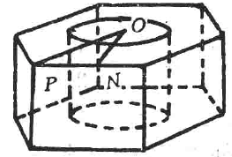
\includegraphics[scale=.5]{fig/2-ex2.png}
    \captionof*{figure}{（第7题）}
\end{minipage}\hfill
\begin{minipage}{.45\textwidth}
        \centering
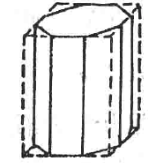
\includegraphics[scale=.5]{fig/2-ex3.png}
    \captionof*{figure}{（第8题）}
\end{minipage}


\item 如图，将正四棱柱底面的边三等分，过三等分点用平行于侧棱的平面截去四个三棱柱，得到一个八棱柱，这个八棱柱的体积是原四棱柱体积的几分之几？
\item 
一圆柱的轴截面为正方形，这个正方形对角线的长为4，求这圆柱的体积.
\end{enumerate}


\section{棱锥、圆锥的体积公式}

上一节我们推导柱体体积公式是分两步进行的；第一步先找出一个特殊的柱体——长方体，根据公理5它的体积公式是$V_{\text{长方体}}=Sh$. 第二步，再根据公理6的推论1推出一般柱体的体积公式是$V_{\text{柱体}}=Sh$. 现在我们要推导锥体的体积公式是否也可以分两步完成呢？那么第一步选取哪个特殊的锥体呢？

我们知道棱柱和棱锥之间有这种关系：一个三棱柱，在保持各棱完整的前提下可以切割成三个三棱锥，如图2.91
\begin{figure}[htp]
    \centering
\begin{tikzpicture}[very thick]

\begin{scope}[xshift=-1cm]
    \tkzDefPoints[]{0/0/A, 2/0/C, 1.3/-.7/B, .5/2.5/A'}
\tkzDefPointsBy[translation=from A to A'](B,C){B',C'}
\tkzDrawPolygon[](A,B,C,C',A',A)
\tkzDrawSegments(A',B A',B' B',C' B',C B',B)
\tkzDrawSegments[dashed](A,C A',C)
\tkzLabelPoints[left](A,A')
\tkzLabelPoints[right](C,C',B')
\tkzLabelPoints[below](B)
\end{scope}
\begin{scope}[xshift=3.5cm]
    \tkzDefPoints[]{0/0/A, 2/0/C, 1.3/-.7/B, .5/2.5/A'}
\tkzDefPointsBy[translation=from A to A'](B,C){B',C'}
\tkzDrawPolygon[](A,B,C,A')
\tkzDrawSegments(A',B)
\tkzDrawSegments[dashed](A,C)
\tkzLabelPoints[left](A,A')
\tkzLabelPoints[right](C)
\tkzLabelPoints[below](B)
\node at (.5,1){1};
\end{scope}
\begin{scope}[xshift=5cm]
    \tkzDefPoints[]{0/0/A, 2/0/C, 1.3/-.7/B, .5/2.5/A'}
\tkzDefPointsBy[translation=from A to A'](B,C){B',C'}
\tkzDrawPolygon[](B,C,B',A')
\tkzDrawSegments(B',B)
\tkzDrawSegments[dashed](A',C)
\tkzLabelPoints[left](A')
\tkzLabelPoints[right](C,B')
\tkzLabelPoints[below](B)
\node at (1.2,1){2};

\end{scope}
\begin{scope}[xshift=6.75cm]
    \tkzDefPoints[]{0/0/A, 2/0/C, 1.3/-.7/B, .5/2.5/A'}
\tkzDefPointsBy[translation=from A to A'](B,C){B',C'}
\tkzDrawPolygon[](C,C',A')
\tkzDrawSegments(A',B' B',C' B',C)
\tkzLabelPoints[left](A')
\tkzLabelPoints[right](C,C',B')
\node at (2,1){3};

\end{scope}
\end{tikzpicture}
    \caption{}
\end{figure}


而三棱柱的体积是这三个三棱锥体积的和.
\[
V_{ABC-A'B'C'}=V_{A'-BB'C}+V_{A'-B'C'C}+V_{A'-ABC} \tag{1}\]
我们来看这三个三棱锥的体积有什么关系.

\noindent
\begin{minipage}{.65\textwidth}\CTEXindent
$\because \quad A'-BB'C$ 与 $A'-B'C'C$ 是等底面积等高.

$\therefore\quad V_{A'-BB'C}=V_{A'-B'C'C}$.

而$A'-BB'C$ 又可看作$C-A'BB'$, 并且$C-ABB'$ 与$C-A'AB$ 是等底面积等高的.

$\therefore\quad V_{C-A'BB'}=V_{C-A'AB}$.

即这三个三棱锥的体积相等， 

$\therefore\quad$ 每个三棱锥的体积是这三棱柱体积的$\frac{1}{3}$. 由此我们得到求三棱锥体积的方法如下：
\end{minipage}\hfill
\begin{minipage}{.3\textwidth}
        \centering
\begin{tikzpicture}
    \tkzDefPoints[]{0/0/A, 2/.45/C, 1.3/-.45/B, 0/2.75/A'}
\tkzDefPointsBy[translation=from A to A'](B,C){B',C'}
\tkzDrawPolygon[](A,B,C,C',A',A)
\tkzDrawSegments(A',B A',B' B',C' B',C B',B)
\tkzDrawSegments[dashed](A,C A',C)
\tkzLabelPoints[left](A,A')
\tkzLabelPoints[right](C,C',B')
\tkzLabelPoints[below](B)
\fill[pattern=north east lines](B)--(C)--(C')--(B')--(B);
\end{tikzpicture}
        \captionof{figure}{}
\end{minipage}

设三棱锥$A'-ABC$ 的底面积是$S$，高是$h$，求它的体积.

\begin{solution}
过$B$、$C$分别作$AA'$ 的平行线$BB'$、$CC'$, 且取$BB'=  CC'=AA'$，连结 $A'B'$、$B'C'$、$C'A'$，则多面体$A'B'C'-ABC$ 是一个三棱柱（图2.92），也就是在三棱锥$A'-ABC$ 上补了一个四棱锥$A-BCC'B'$，就成了一个三棱柱，它的底仍是$\triangle ABC$，高还是$A'-ABC$ 的高即是$h$.

$\therefore\quad V_{A'B'C'-ABC}=Sh$.

连结$B'C$, 则$S_{\triangle B'BC}=S_{\triangle B'C'C}$,

$\therefore\quad V_{A'-B'BC}=V_{A'-B'C'C}$, 再看四棱锥$D-A'ABB'$，它被面$A'BC$ 分成了体积相等的两部分，即$V_{C-A'AB}=V_{C-A'BB'}$.

而$C-A'AB$ 就是三棱锥$A'-ABC$，
$C-ABB'$ 就是三棱锥$A'-BB'C$.

$\therefore\quad V_{A'-ABC}=V_{A'-BB'C}=V_{A'-B'C'C}=\frac{1}{3}V_{ABC-A'B'C'}=\frac{1}{3}Sh$.
\end{solution}

这就得到下面的定理：

\begin{thm}
    {定理} 如果三棱锥的底面积是$S$，高是$h$，那么它的体积是
    \[V_{\text{三棱锥}}=\frac{1}{3}Sh\]
\end{thm}


因为和一个三棱锥等底面积等高的任何锥体都和这三棱锥的体积相等，所以得到下面的定理.
\begin{thm}
{定理} 如果一个锥体（棱锥、圆锥）的底面积是$S$，高是$h$，那么它的体积是
\[
V_{\text{锥体}}=\frac{1}{3}Sh\]    
\end{thm}

\begin{thm}
 {推论} 如果圆锥的底面半径是$r$，高是$h$，那么它的体积是
\[V_{\text{圆锥}}=\frac{1}{3}\pi r^{2} h   \]
\end{thm}


\noindent
\begin{minipage}{.65\textwidth}
\begin{example}
如图2.93，已知：三棱锥$A-BCD$的侧棱$AD$垂直于底面$BCD$，侧面$ABC$是边长为$a$的等边三角形且与底面所成的角为$\theta$.

求证： $V_{\text{三棱锥}}=\frac{1}{16}a^{3}\sin2\theta$.    
\end{example}

\begin{analyze}
    因棱锥的高$AD$已知，易作出侧面与底面所成二面角的平面角$AED$. 由于$AB=AC=BC=a$, 所以$BC$边上的高$AE$可求. 从而$AD$的大小、$\triangle BCD$中$BC$边上的高$DE$都可求出. 从而可求出底面积和高，进而可求$V$.
\end{analyze}    
\end{minipage}\hfill
\begin{minipage}{.3\textwidth}
    \centering
\begin{tikzpicture}[very thick]
\tkzDefPoints{0/0/B, 3/0/D, 1.2/-1.3/C, 3/2.5/A}
\tkzDefMidPoint(B,C)  \tkzGetPoint{E}
\tkzDrawPolygon[](A,B,C,D)
\tkzDrawSegments(A,E A,C)
\tkzDrawSegments[dashed](B,D E,D)
\node at (1,-.45){$\theta$};
\tkzLabelPoints[left](B,E)
\tkzLabelPoints[right](D,A,C)
\end{tikzpicture}
\captionof{figure}{}
\end{minipage}



\begin{proof}
 在平面$BCD$内，作$DE\perp BC$, 垂足为$E$，连结$AE$ 
 
$\because\quad  AD\perp \text{底面} BCD$,  

$\therefore\quad  DE$就是$AE$在平面$BCD$上的射影. 根据三垂线定理， $AE\perp BC$.

$\therefore\quad \angle AED=\theta$,   

\[\begin{split}
    V_{\text{三棱锥}}&=\frac{1}{3}S_{\triangle BOD}\cdot  AD\\
    & =\frac{1}{3}\x \frac{1}{2}BC\cdot  ED\cdot AD\\
    &=\frac{1}{3}\x\frac{1}{2}BC\cdot  AE\cos\theta\cdot AE\sin\theta\\
    & =\frac{1}{6}a\cdot \frac{\sqrt{3}}{2}a\cdot \cos\theta\cdot \frac{\sqrt{3}}{2}a\cdot \sin\theta\\
    & =\frac{1}{16}a^{3}\sin2\theta
\end{split}\]
\end{proof}

\begin{example}
    一块正方形薄铁板的边长是22cm，以它的一个顶点为圆心，边长为半径画弧，沿弧剪下一个扇形. 用这块扇形铁板围成一个圆锥筒，求它的容积（保留两位有效数字）.
\end{example}

\begin{figure}[htp]
    \centering
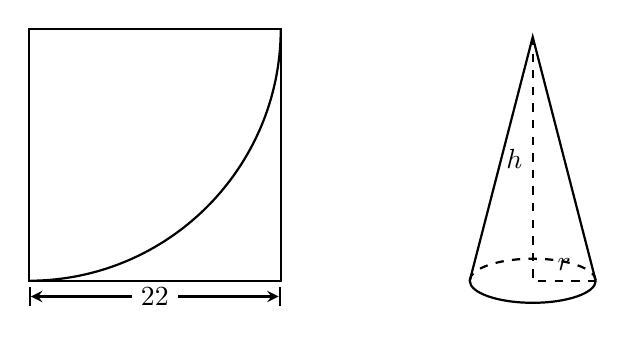
\begin{tikzpicture}[thick, >=stealth, scale=.8]
    \begin{scope}
\draw[|<->|](0,-.25)--node[fill=white]{22}(4,-.25);
\draw(0,0) rectangle (4,4);
\draw(0,0) arc (-90:0:4);

\end{scope}
\begin{scope}[xshift=8cm]
\draw(1,0)--(0,3.87)--(-1,0);
\draw[dashed](0,3.87)--node[left]{$h$}(0,0)--node[above]{$r$}(1,0);
\draw(-1,0) arc [start angle = -180, end angle =0, x radius = 1, y radius = .35];
\draw[dashed](-1,0) arc [start angle = 180, end angle =0, x radius = 1, y radius = .35];
\end{scope}
\end{tikzpicture}
    \caption{}
\end{figure}

\begin{analyze}
    求圆锥筒的容积，即
求这圆锥的体积. 这圆锥的侧面即剪下的那个扇形.
\end{analyze}

\begin{solution}
    如图2.94，扇形弧长是$\frac{1}{4}\cdot 2\pi\cdot 22=\frac{1}{4}\cdot 44\pi=11\pi$. 因此，所作的圆锥筒底的周长 $2\pi r=11\pi$.
解得$r=5.5$.

因为母线长是22cm，所以圆锥的高
\[h=\sqrt{22^{2}-5.5^{2}}\approx 21.3\]
\[V_{\text{圆锥}}=\frac{1}{3}\pi\x 5.5^{2}\x 21.3
\approx 6.7\x  10^{2}\left(\mathrm{cm}^{3}\right)\]

答：所求圆锥筒的容积约为$670\mathrm{cm}^{3}$.
\end{solution}


\begin{example}
    如图2.95，三棱锥$P-ABC$中，若$PA\perp BC$,  $PA= BC=\ell$,  $PA$、$BC$的公垂线段$ED=h$，求$V_{P-ABC}$.
\end{example}

\begin{analyze}
$\because\quad ED\perp PA,\quad  BC\perp PA,\quad  ED\cap BC=D$,

$\therefore\quad PA\perp \text{平面}BEC$. $PE$和$AE$分别是三棱锥$P-EBC$, $A-EBC$的高. 

由已知易求$S_{\triangle BEC}$.    
\end{analyze}

\begin{solution}
连结$EB$、$EC$.

$\because\quad PA\perp BC, \quad PA\perp ED,\quad  BC\cap ED=D$, 

$\therefore PA\perp \text{平面}EBC$.

\noindent
\begin{minipage}{.6\textwidth}\CTEXindent
\[\begin{split}
V_{P-ABC}&=V_{P-EBC}+V_{A-EBC}\\
&=\frac{1}{3}\cdot  AE\cdot  S_{\triangle EBC}+\frac{1}{3}\cdot  PE\cdot  S_{\triangle EBC}\\
&=\frac{1}{3}(AE+PE)S_{\triangle EBC}\\
&=\frac{1}{3}\cdot  AP\cdot  S_{\triangle EBC}\\
&=\frac{1}{3}\cdot  \ell\cdot \frac{1}{2}h\ell\\
&=\frac{1}{6}h\ell^{2}.    
\end{split}\]    
\end{minipage}
\hfill
\begin{minipage}{.35\textwidth}
\begin{tikzpicture}[very thick]
\tkzDefPoints{0/0/A, 4/0/C, 1.2/-1.25/B, 2.25/2.5/P}
\tkzDrawPolygon(A,B,C,P)

\tkzDefPointWith[linear, K=.3](A,P)  \tkzGetPoint{E}
\tkzDefPointWith[linear, K=.26](B,C)  \tkzGetPoint{D}

\tkzDrawSegments(E,B B,P)
\tkzDrawSegments[dashed](A,C E,D E,C)
\tkzLabelPoints[left](A,E)
\tkzLabelPoints[right](P,C)
\tkzLabelPoints[below](B,D)

\end{tikzpicture}
\captionof{figure}{}
\end{minipage}
\end{solution}



\begin{thm}
{思考题：}
例2.42还有别的解法吗？试给出你的思路.    
\end{thm}





\begin{example}
在棱长为$a$的正方体$ABCD-A_{1}B_{1}C_{1}D_{1}$ 中，求面对角线$A_{1}C_{1}$ 与 $B_{1}C$ 的距离（图2.96）.    
\end{example}

\begin{figure}[htp]
    \centering
\begin{tikzpicture}[thick, scale=.9]
\tkzDefPoints{0/0/B, 3/0/C, 3.9/.9/D, 0/3/B_1}
\tkzDefPointsBy[translation=from C to D](B){A}
\tkzDefPointsBy[translation=from B to B_1](A,C,D){A_1,C_1,D_1}
\tkzDrawPolygon(B,C,D,D_1,A_1,B_1)
\tkzDrawSegments[dashed](A,C A,B_1 A_1,C A,D A,B A,A_1)
\tkzDrawSegments(B_1,C_1 C_1,D_1 A_1,C_1 B_1,C C,C_1)
\tkzLabelPoints[left](B,B_1,A_1,A)
\tkzLabelPoints[right](C,D,C_1,D_1)

\end{tikzpicture}
    \caption{}
\end{figure}

\begin{solution}
    连结$AB_{1}$、$AC$、$A_{1}C$.

$\because\quad A_{1}C_{1}\parallel AC$,

$\therefore\quad A_{1}C_{1}\parallel \text{平面} ACB_{1}$. $A_{1}C_{1}$ 与 $B_{1}C$ 的距离就是三棱锥 $V_{A_{1}-ACB_{1}}$ 的高.

$\because\quad \frac{1}{3}\cdot  h\cdot  S_{\triangle AB_{1}C}=V_{A_{1}-ACB_{1}}=V_{C-A_{1}AB_{1}}=\frac{1}{3}\cdot S_{\triangle A_{1}AB_{1}}\cdot BC$,

$\therefore\quad h\cdot\frac{\sqrt{3}}{4}\left(\sqrt{2}a\right)^{2}=\frac{1}{2}a^{2}\cdot a$,

\[h=\frac{\sqrt{3}}{3}a\]
\end{solution}

\begin{remark}
\begin{enumerate}
    \item  由于棱锥（或圆锥）的体积是与其同底等高的棱柱（或圆柱）体积的三分之一，因此，求棱锥的体积可转化为求同底等高的棱柱的体积.

    \item  若一个几何体的体积不易直接求出，而它可分割成几个简单的几何体，则该几何体的体积是这几个简单体的体积之和.

    \item 同一个几何体的体积若从两个不同的角度去计算，则它们的值相等.这不仅提示我们可换个角度去研究问题，又常常以这个等量关系作为构造方程的依据.
\end{enumerate}
\end{remark}

\subsection*{2.9 练习}
\begin{enumerate}
    \item 如图：将平行六面体沿相邻三个面的对角线截去一个三
棱锥，则这个三棱锥的体积是平行六面体体积的$\underline{\qquad\qquad}$.

\noindent
\begin{minipage}{.48\textwidth}
    \begin{center}
\begin{tikzpicture}[very thick]
\tkzDefPoints{0/0/A, 3/0/B, -1/1.5/D, .6/1/A'}
\tkzDefPointsBy[translation=from A to D](B){C}
\tkzDefPointsBy[translation=from A to A'](B,C,D){B',C',D'}
\tkzDrawPolygon(A,B,B',C',D',D)
\tkzDrawSegments[dashed](C',D C,D B,C C,C')
\tkzDrawSegments(A,A' A',D' A',B' D,A' A',C')
\fill[pattern = north east lines](A')--(C')--(D)--(A');
\end{tikzpicture}
\captionof*{figure}{（第1题）}    
\end{center}
\end{minipage}\hfill
\begin{minipage}{.48\textwidth}
    \begin{center}
\begin{tikzpicture}
\tkzDefPoints{0/0/A', 3/0/B, 1/.7/D, 0/3/A}
\tkzDefPointsBy[translation=from A' to D](B){C'}
\tkzDefPointsBy[translation=from A' to A](B,C',D){B',C,D'}
\tkzDrawPolygon(A',B,C',C,D',A)
\tkzDrawSegments[dashed](A',D D,C' D,B C,D A,D D,D')
\tkzDrawSegments(C,A A,B C,B A,B' B,B' C,B')
\tkzLabelPoints[left](A)
\tkzLabelPoints[right](B,C)
\tkzLabelPoints[below](D)
\end{tikzpicture}
\captionof*{figure}{（第2题）}    
\end{center}
\end{minipage}

\item 一个各棱长都相等的正三棱锥，可以从一个正方体如第 2题图那样截去四个三棱锥而得到，若正方体的棱长为$a$，则所得正三棱锥的体积是$\underline{\qquad\qquad}$；若这正三棱锥的棱长为$a$，这正三棱锥的体积是$\underline{\qquad\qquad}$.

\item 利用第2题的图，各棱长都是$a$的正三棱锥的高是$\underline{\qquad\qquad}$，相对两棱的距离是$\underline{\qquad\qquad}$.  
\item 
在下列情形下，正棱锥体积变化以后与变化以前体积的比是(1) $\underline{\qquad\qquad}$；(2)$\underline{\qquad\qquad}$
\begin{enumerate}[(1)]
    \item 高和底面边长都增为原来的$n$倍；
    \item 高增为原来的$n$倍，底面边长缩为原来的$\frac{1}{n}$.
\end{enumerate}

\item 已知下列各正棱锥的底面边长是$a$，侧棱长是$b$. 求它的体积：
\begin{enumerate}[(1)]
    \item 正三棱锥$V=\underline{\qquad\qquad}$.
    \item 正四棱锥$V= \underline{\qquad\qquad}$.
    \item 正六棱锥$V= \underline{\qquad\qquad}$.
\end{enumerate}

\item 三棱锥的三个侧面互相垂直，它们的面积分别为$6\mathrm{m}^{2}$,  $4\mathrm{m}^{2}$ 和$3\mathrm{m}^{2}$. 则它的体积是$\underline{\qquad\qquad}$.  

\item 棱锥被平行于底面的平面截得的小棱锥的体积和原来棱锥的体积的比，等于它们的高的$\underline{\qquad\qquad}$比.


\noindent
\begin{minipage}{.6\textwidth}
\item 已知：圆锥的底面周长是$c$，高是$h$.

求证：这个圆锥的体积$V$可以近似地表示为
\[V\approx \left(\frac{c}{6}\right)^{2}h\]


\item 如图，$P$为矩形$ABCD$的$CD$
边上的任一点，当矩形绕轴$AB$旋转一周时，$\triangle ABP$、 $\triangle ADP$、$\triangle BPC$旋转所成的旋转体的体积分别是$V_{1}$、$V_{2}$、$V_{3}$, 那么$\frac{V_{1}}{V_{2}+V_{3}}$的值是$\underline{\qquad\qquad}$.    
\end{minipage}\hfill
\begin{minipage}{.28\textwidth}
    \centering
\begin{tikzpicture}[thick, scale=.8]
    \tkzDefPoints{0/0/B, 3/0/C, 0/4/A, 3/4/D, 3/3/P}
\tkzDrawPolygon(A,B,C,D)
\tkzDrawSegments[](A,P B,P)
\tkzLabelPoints[left](A,B)
\tkzLabelPoints[right](C,D,P)
\end{tikzpicture}
\captionof*{figure}{（第9题）}
\end{minipage}


\end{enumerate}


\section{棱台、圆台的体积公式}
我们知道，棱台、圆台分别是由棱锥和圆锥用平行于底面的平面截去一个锥体而得到的. 既然锥体体积公式已经知道了，台体的体积就可用两个锥的体积之差推导出来.

如果台体（棱台或圆台）的上、下底面面积分别是$S$和$S'$，高是$h$，求这台体的体积.

\begin{analyze}
    只要补出形成台体的锥体，则台体的体积应是大锥体的体积与截去的小锥体的体积之差.
\end{analyze}

\begin{figure}[htp]
    \centering
\begin{tikzpicture}[scale=1.4]
\tkzDefPoints{1/.5/S, 1/1.5/S'}
\draw[dashed](S') ellipse[x radius=.6, y radius=.2];
\draw[dashed](S) ellipse[x radius=1, y radius=.3];
\tkzDefPoints{0/.5/A_2, .4/1.5/A_1, 2/.5/B_2, 1.6/1.5/B_1}
\tkzInterLL(A_1,A_2)(B_1,B_2)  \tkzGetPoint{H}
\tkzDrawSegments(A_2,H  B_2,H)
\draw(A_2) arc [start angle =-180, end angle =0, x radius=1, y radius=.3];
\draw(A_1) arc [start angle =-180, end angle =0, x radius=.6, y radius=.2];
\tkzDrawSegments[dashed](H,S)    
\tkzLabelPoints[left](S',S)
\tkzLabelSegment[right](S',S){$h$}
\tkzLabelSegment[right](S',H){$x$}


\tkzDefPoints{3/0.5/A, 5/0.5/C, 3.6/-.1/B, 4.2/1.1/D, 4/3/G, 4/0.5/S}

\foreach \x in {A,B,C,D,S}
{
    \tkzDefPointWith[linear, K=.63](G,\x) \tkzGetPoint{\x'}
}

\tkzDrawPolygon(G,A,B,C)
\tkzDrawSegments[dashed](G,D G,S C,D D,A C',D' D',A')

\tkzDrawSegments(A',B' B',C' G,B)

\tkzLabelSegment[left](S,S'){$h$}
\tkzLabelSegment[right](S',G){$x$}
\tkzLabelPoint[right](S){$S$}
\tkzLabelPoint[right](S'){$S'$}

\tkzDefPoints{-1.5/-.5/a, 4.5/-.5/b, 6/1.25/c}
\tkzDefPointsBy[translation = from b to c](a){d}

\tkzDrawSegments(a,b b,c d,a)
\tkzInterLL(c,d)(H,A_1) \tkzGetPoint{tmp1}
\tkzInterLL(c,d)(H,B_2) \tkzGetPoint{tmp2}
\tkzInterLL(c,d)(G,A') \tkzGetPoint{tmp3}
\tkzInterLL(c,d)(G,C') \tkzGetPoint{tmp4}

\tkzDrawSegments(c,tmp4 tmp3,tmp2 tmp1,d)
\tkzDrawSegments[dashed](tmp4,tmp3 tmp2,tmp1)
\tkzDrawPoints(S,S')

\node at (-1.3,-.5)[above right]{$\alpha$};


\end{tikzpicture}
    \caption{}
\end{figure}


\begin{solution}
设截得台体时去掉的锥体的高是$x$（图2.97），则截得这个台体的锥体的高是$h+x$, 
\[\begin{split}
    V_{\text{台体 }}&=V_{\text{大锥体 }}-V_{\text{小锥体 }}\\
&=\frac{1}{3}S(h+x)-\frac{1}{3}S'x\\
&=\frac{1}{3}\left[Sh+\left(S-S'\right)x\right]
\end{split}\]

下面，我们用$S$、 $S'$、 $h$来表示$x$. 由锥体的性质得
\[\frac{S'}{S}=\frac{x^{2}}{(h+x)^{2}}\]
$\therefore\quad \frac{\sqrt{S'}}{\sqrt{S}}=\frac{x}{h+x},\quad x=\frac{\sqrt{S'}h}{\sqrt{S}-\sqrt{S'}}.$

代入上式，得
\[\begin{split}
V_{\text{台体 }}&=\frac{1}{3}h\left[S+\left(S-S'\right)\frac{\sqrt{S'}}{\sqrt{S}-\sqrt{S'}}\right]\\
& =\frac{1}{3}h\left[S+\sqrt{S'}(\sqrt{S}+\sqrt{S'})\right]\\
& =\frac{1}{3}h\left[S+\sqrt{SS'}+S'\right].    
\end{split}\]
\end{solution}

由此我们得到下面的定理：
\begin{thm}
{定理} 如果台体（棱台、圆台）的上、下底面的面积分别是$S'$、 $S$，高是$h$，那么它的体积是
\[V_{\text{台体 }}=\frac{1}{3}h\left(S+\sqrt{SS'}+S'\right)
\]
\end{thm}

\begin{thm}
 {推论} 如果圆台的上、下底面半径分别是$r'$、 $r$，高是$h$，那么它的体积是
\[ V_{\text{圆台 }}=\frac{1}{3}\pi h\left(r^{2}+rr'+r^{\prime 2}\right)
 \]
\end{thm}

像柱体、锥体、台体的测面积公式之间的关系一样，它们的体积公式之间，也有类似地关系. 如下图.
\begin{figure}[htp]
    \centering
\begin{tikzpicture}[>=stealth, thick]
\node[draw] (A) at (0,3) {$V_{\text{台体 }}=\frac{1}{3}h\left(S+\sqrt{SS'}+S'\right)$};
\node[draw] (B1) at (-2, 1.5) {$S'=S$};
\node[draw] (B2) at (2, 1.5) {$S'=0$};
\node[draw] (C1) at (-2, 0) {$V_{\text{柱体 }}=Sh$};
\node[draw] (C2) at (2, 0) {$V_{\text{锥体 }}=\frac{1}{3}Sh$};
\draw[->](A)--(B1);
\draw[->](A)--(B2);
\draw[->](B1)--(C1);
\draw[->](B2)--(C2);
\end{tikzpicture}
\end{figure}

\noindent
\begin{minipage}{.7\textwidth}\CTEXindent
    \begin{example}
    一个圆环铁片，它的内圆半径为45cm，外圆半径
是75cm，用它的$\frac{1}{3}$ 作圆台形水桶的侧面，这个水桶容积是多少？
\end{example}

\begin{analyze}
 水桶的容积即是它的体积. 圆环形铁片是圆台形水桶的侧面，所以这圆台上、下底面
圆的周长分别是内外圆周长的$\frac{1}{3}$. 圆台的母线长就是圆环外圆和内圆半径的差. 而圆台的高可通过上、下底的半径及母线长求出.   
\end{analyze}
\end{minipage}\hfill 
\begin{minipage}{.25\textwidth}
    \centering
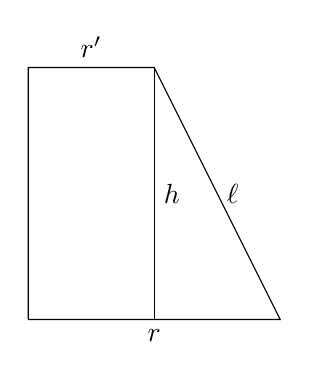
\begin{tikzpicture}[scale=.8]
\draw(0,0)--node[below]{$r$}(4,0)--node[right]{$\ell$}(2,4)--node[above]{$r'$}(0,4)--(0,0);
\draw(2,4)--node[right]{$h$}(2,0);
\end{tikzpicture}
\captionof{figure}{}
\end{minipage}

\begin{solution}
这个圆台上底周长是$c'=\frac{1}{3}\x  2\pi\x 45$,

$\therefore\quad $圆台上底半径是$r'=\frac{c'}{2\pi}=15(\mathrm{cm})$.

同理，圆台下底半径 $r=25(\mathrm{cm})$.
而圆台侧面母线长$\ell=75-45=30(\mathrm{cm})$,

$\therefore\quad$ 圆台的高 
\[\begin{split}
h&=\sqrt{\ell^{2}-\left(r-r'\right)^{2}}\\
&=\sqrt{30^{2}-10^{2}}\\
&=20\sqrt{2}(\mathrm{cm}).    
\end{split}\]

\[\begin{split}
\therefore\quad V_{\text{圆台 }}&=\frac{1}{3}\pi h\left(r^{2}+rr'+r^{\prime 2}\right)\\
&=\frac{1}{3}\pi\cdot 20\sqrt{2}(625+375+225)\\
&\approx 8167\sqrt{2}\pi \left(\mathrm{cm}^{3}\right)    
\end{split}\]
\end{solution}


\subsection*{2.10 练习}

一、选择题
\begin{enumerate}
    \item 边长为1的正方形$ABCD$中，$E$、$F$分别是$BC$、$DC$的中点，使$C$、$B$、$D$重合，把$ABCD$沿$AE$、$EF$、$FA$折起组成一个四面体，这个四面体的体积为 \hfill (\qquad )
\begin{multicols}{4}
\begin{enumerate}[(A)]
\item $\frac{1}{8}$.
\item $\frac{1}{24}$.
\item $\frac{\sqrt{2}}{24}$.
\item $\frac{\sqrt{5}}{48}$.
\end{enumerate}
\end{multicols}

\item 正四棱锥底面面积为$Q$，侧面积为$S$，则它的体积为\hfill (\qquad )
\begin{multicols}{2}
\begin{enumerate}[(A)]
\item $\frac{1}{3}Q\sqrt{S}$.
\item $\frac{1}{2}\sqrt{Q\left(S^{2}-Q^{2}\right)}$.
\item $\frac{1}{2}\sqrt{S\left(S^{2}-Q^{2}\right)}$.
\item $\frac{1}{6}\sqrt{a\left(S^{2}-Q^{2}\right)}$.
\end{enumerate}
\end{multicols}
\item 一个棱锥被平行于底面的平面所截，如果截面面积和底面面积的比是1:2，那么这截面所截得的棱锥与原来棱
锥体积的比是\hfill (\qquad )
\begin{multicols}{4}
\begin{enumerate}[(A)]
\item $1:2$.
\item $1:\sqrt{2}$.
\item $1:2\sqrt{2}$.
\item $1:(\sqrt{2}-1)$.
\end{enumerate}
\end{multicols}


\item 一个圆环内外半径分别为4和6，一直径把它分成两部分，以其中的一部分-扇环所卷成的圆台的体积是\hfill (\qquad )
\begin{multicols}{4}
\begin{enumerate}[(A)]
\item $168\sqrt{3}\pi $.
\item $84\sqrt{3}\pi$.
\item $72\sqrt{3}\pi $.
\item $56\sqrt{3}\pi$.
\end{enumerate}
\end{multicols}

\item 棱台上、下底面面积的比是1:9，则此棱台中截面把棱台分成的两部分的体积的比是 \hfill (\qquad )
\begin{multicols}{4}
\begin{enumerate}[(A)]
\item $1:7$.
\item $2:7$.
\item $7:19$.
\item $3:16$.
\end{enumerate}
\end{multicols}

\item 连结四面体各棱的中点得到一个内接于这四面体的八面体，则这八面体与原四面体体积之比是 \hfill (\qquad )
\begin{multicols}{4}
\begin{enumerate}[(A)]
\item $2:3$.
\item $2:5$.
\item $3:4$.
\item $1:2$.
\end{enumerate}
\end{multicols}


\item 表面积为$A$的多面体的每个面都外切于表面积为$36\pi$ 的一个球，则这多面体的体积是 \hfill (\qquad )
\begin{multicols}{4}
\begin{enumerate}[(A)]
\item $\frac{A}{3}$.
\item $\frac{A}{2}$.
\item $A$.
\item $A^2$.
\end{enumerate}
\end{multicols}
\end{enumerate}

二、填空题：
\begin{enumerate}
    \item 在棱台$ABC-A_{1}B_{1}C_{1}$ 中，若$V_{B_1-ABC}=4$,  $V_{B-A_{1}B_{1}C_{1}}=16$, 则这个棱台的体积是$\underline{\qquad\qquad}$.

    \item 两底面边长分别是15m、10m的正三棱台，它的侧面积等于两底面面积的和，则这个三棱台的体积是$\underline{\qquad\qquad}$.

    \item 圆台的高为3，一个底面半径是另一个底面半径的2倍，母线与下底面所成的角为$45^{\circ}$. 它的体积是$\underline{\qquad\qquad}$.

\item 圆台的体积是$234\sqrt{3}\pi\mathrm{cm}^{3}$，侧面展开图是半圆环，它的大半径等于小半径的3倍，这个圆台的上底面半径是$\underline{\qquad\qquad}$.

\item 圆台的母线长为6cm，它和下底面夹角为$60^{\circ}$, 又轴截面的两条对角线互相垂直，这圆台的体积为$\underline{\qquad\qquad}$.

\item 一个正四棱台，上、下底面边长分别为2cm和6cm，侧面与底面成$60^{\circ}$ 角，则它的侧面积$S=\underline{\qquad\qquad}$. 体积 $V=\underline{\qquad\qquad}$.

\item 圆台的两底面半径分别是$a$和$b$ ($a>b$)，求这圆台的体积与截得它的圆锥的体积的比。
\end{enumerate}


\section*{习题六}

\begin{center}
    \bfseries A
\end{center}

\begin{enumerate}
    \item 
斜三棱柱$ABC-A_{1}B_{1}C_{1}$ 的底面是边长为$a$的正三角形，侧棱长为$b$，侧棱$AA_{1}$ 与底面两边AB、AC都成$60^{\circ}$ 角.求这个三棱柱的侧面积和体积.

\noindent
\begin{minipage}{.6\textwidth}
   \item 三棱柱各侧棱间距离的比为$9:10:17$，侧棱长为1cm, 侧面积为$6\mathrm{cm}^{2}$, 求这个棱柱的体积。
   \item 已知一斜棱柱的底面是梯形，求证它的体积等于两个平行侧面面积之和与这两个平行侧面之间的距离的乘积之半.
\item 经过正三棱柱底面一边$AB$，作与底面成$30^{\circ}$ 角的平面，已知截面$\triangle ABD$的面积为$32\mathrm{cm}^{2}$, 求截得的三棱锥$D-ABC$的体积.    
\end{minipage}\hfill
\begin{minipage}{.3\textwidth}
\centering
    \begin{tikzpicture}[thick, scale=.8]
\tkzDefPoints{0/0/C, 3/0/B, 2/-1/A, 0/4/C', 0/1.5/D}
\tkzDefPointsBy[translation=from C to C'](A,B){A',B'}
\tkzDrawPolygon(C,A,B,B',C')
\tkzDrawSegments[dashed](B,C D,B)
\tkzDrawSegments(A',C' A',B' A,A' A,D)
\tkzLabelPoints[left](C,D)
\tkzLabelPoints[right](A,B)

\end{tikzpicture}
\captionof*{figure}{（第4题）}
\end{minipage}

\end{enumerate}

\begin{center}
    \bfseries B
\end{center}

\begin{enumerate}\setcounter{enumi}{4}
    \item 已知四面体$ABCD$，棱$AB=a$,  $CD=b$,  $AB$与$CD$间的距离为$d$，所成的角为$90^{\circ}$.
\begin{enumerate}[(1)]
    \item 求这四面体的体积；
    \item 
若这四面体被平行于棱$AB$、$CD$的平面$\alpha$截成两部分，设$AB$、$CD$到平面$\alpha$的距离之比为$k$，求证：这四体被平面$\alpha$分成的两部分体积之比是 $\frac{k^{2}(k+3)}{3k+1}$.
\end{enumerate}

\noindent
\begin{minipage}{.45\textwidth}
\centering
\begin{tikzpicture}[very thick]
\tkzDefPoints{0/0/B, 3/0/D, 2/-.7/C, 2.2/2/A}
\tkzDrawPolygon(A,B,C,D)
\tkzDrawSegments(A,C)
\tkzDrawSegments[dashed](B,D)
\tkzLabelPoints[left](B)
\tkzLabelPoints[right](D)
\tkzLabelPoints[below](C)
\tkzLabelPoints[above](A)
\end{tikzpicture}
\captionof*{figure}{（第5题）}
\end{minipage}\hfill
\begin{minipage}{.45\textwidth}
\centering
\begin{tikzpicture}[very thick]
\tkzDefPoints{0/0/A, 3/0/B, 4/1.2/C, 2/4/S}
\tkzDefPointsBy[translation=from B to C](A){D}
\tkzDefPointWith[linear, K=.45](S,C)
\tkzGetPoint{E}
\tkzDrawPolygon(A,B,C,S)
\tkzDrawSegments(B,S B,E)
\tkzDrawSegments[dashed](B,D C,D A,D S,D D,E)
\tkzLabelPoints[left](A)
\tkzLabelPoints[right](B,C,E)
\tkzLabelPoints[below](D)
\tkzLabelPoints[above](S)    
\end{tikzpicture}
\captionof*{figure}{（第6题）}
\end{minipage}

\item 正四棱锥$S-ABCD$的底面边长为$a$，底面边长与侧棱之比为$\sqrt{3}:\sqrt{2}$, 过底面一对角线$BD$作平行于侧棱$SA$的截面$EBD$. 试求：
\begin{enumerate}[(1)]
   \item 截面与底面$ABCD$所成二面角的度数；
    \item 被截面$EBD$所截得的三棱锥$E-BDC$的体积.
\end{enumerate}


\item 经过圆锥顶点$P$的一个截面$PAB$和底面成$60^{\circ}$ 的二面角，
且截底面圆得$ 120^{\circ} $的$ \wideparen{AB}$. 底面圆心$O$到截面$PAB$的距离是30cm，求$P-OAB$的体积。
\item 正三棱台的上底面边长为2cm，过上底一边而平行于一条侧棱的截面，分棱台为体积相等的两部分，求棱台的下底面边长.

\item 已知过三棱台上底面的一边与一条侧棱平行的一个截面，它的两个顶点是下底面两边的中点. 求棱台被分成两部分的体积的比.

\noindent
\begin{minipage}{.45\textwidth}
\centering
\begin{tikzpicture}[very thick]
    \draw(-2,0)--(0,3)node[above]{$P$}--(2,0);
    \draw[dashed](-2,0) arc [start angle =180, end angle =0, x radius =2, y radius=.6];
    \draw (-2,0) arc [start angle =180, end angle =360, x radius =2, y radius=.6];
\tkzDefPoints{0/0/O, .8/-.6/A, 1.25/.5/B}
\draw[dashed](A)--(O)--(B)--(A);
\draw(A)--(0,3);
\draw[dashed](O)--(0,3)--(B);
\tkzLabelPoints[left](O)
\tkzLabelPoints[below](A,B)

\end{tikzpicture}    
\captionof*{figure}{（第7题）}
\end{minipage}\hfill
\begin{minipage}{.45\textwidth}
\centering
\begin{tikzpicture}
\tkzDefPoints{0/0/A, 4/0/B, 1.5/2/C, 1/2.5/A', 3/2.5/B', 1.75/3.5/C'}
\tkzDefMidPoint(A,B) \tkzGetPoint{D}
\tkzDefMidPoint(C,B) \tkzGetPoint{E}
\tkzDrawPolygon(A,B,B',C',A')
\tkzDrawSegments[dashed](A,C B,C C',E C,C' D,E)
\tkzDrawSegments(A',D A',B')
\tkzLabelPoints[left](A,A')
\tkzLabelPoints[above](C')
\tkzLabelPoints[right](C,E,B,B')
\tkzLabelPoints[below](D)
\end{tikzpicture}    
\captionof*{figure}{（第9题）}
\end{minipage}

\end{enumerate}

\begin{center}
    C
\end{center}
\begin{enumerate}\setcounter{enumi}{9}
    \item 如图已知圆柱的轴截面为$AA' B'B$, $C$为圆柱底面圆周上一点，设棱锥$A' -ABC$ 的体积为$V_{\text{锥} }$, 圆柱的体积为$V_{\text{柱 }}$.
且 $\frac{V_{\text{锥 }}}{V_{\text{柱 }}}=\frac{1}{6\pi}$.
\begin{enumerate}[(1)]
\item 求二面角$B-AA' -C$ 的大小；
    \item   若二面角 $A-A' B-C $等于$\alpha$, $\angle BA' C=\beta$，二面角$B-AA' -C$ 等于$\gamma$，求证：$\sin\alpha\cdot \cos\beta=\cos\gamma$
\end{enumerate}

\noindent
\begin{minipage}{.45\textwidth}
\centering
\begin{tikzpicture}[very thick, scale=.9]
\tkzDefPoints{-1.5/0/A', 1.5/0/B', -1.5/4/A, 1.5/4/B, .5/3.6/C}
\draw (0,4) ellipse [x radius  = 1.5, y radius = .5];
\tkzDrawSegments(A,A' B,B' A,C B,C A,B)
\tkzDrawSegments[dashed](A',B' A',B A',C)
\draw[dashed] (A') arc [start angle=180, end angle =0, x radius  = 1.5, y radius = .5];
\draw (A') arc [start angle=180, end angle =360, x radius  = 1.5, y radius = .5];
\tkzLabelPoints[left](A,A')
\tkzLabelPoints[right](B,B')
\tkzLabelPoints[below left](C)


\end{tikzpicture}    
\captionof*{figure}{（第10题）}
\end{minipage}\hfill
\begin{minipage}{.45\textwidth}
\centering
\begin{tikzpicture}
\tkzDefPoints{0/0/A', 1.8/.5/B', 1.3/1.2/C', 0.5/3/A}
\tkzDefPointsBy[translation=from A' to A](B',C'){B,C}
\tkzDrawPolygon(A,C,B,B',A')
\tkzDrawSegments[dashed](A',C' C,C' B',C')
\tkzDrawSegments(A,B)
\tkzLabelPoints[left](A,A')
\tkzLabelPoints[right](B,B',C')
\tkzLabelPoints[above](C)
\end{tikzpicture}    
\captionof*{figure}{（第11题）}
\end{minipage}




\item 斜三棱柱$ ABC-A' B' C'$中，底面$A' B' C'$是正三角形， $\angle AA' B' =\angle AA' C'$:
\begin{enumerate}[(1)]
    \item 求证： $BB' C' C$ 为矩形；
    \item 设$AA'$  与底面$A' B'   C'$的夹角为$45^{\circ}$，侧棱$AA' =b$, $\triangle ABC$的边长为$a$，求棱柱的侧面积和体积。
\end{enumerate}
\end{enumerate}



\section{*拟柱体及其体积公式}

我们知道，图2.99、图2.100所示的多面体，尽管它们有两个面互相平行，但它不是棱台. 下面我们研究这类多面体.

\noindent
\begin{minipage}{.45\textwidth}
    \centering
\begin{tikzpicture}[scale=.8]
\tkzDefPoints{0/0/A, 3/0/B, 4.1/1/C}
\tkzDefPoints{1/3/A', 3/3/B', 3.5/3.3/C'}
\tkzDefPointsBy[translation=from B' to C'](A'){D'}
\tkzDefPointsBy[translation=from B to C](A){D}

\tkzDrawPolygon[](A,B,C,C',D',A')
\tkzDrawSegments[dashed](C,D D,A D,D')
\tkzDrawSegments[](A',B' B',C' B,B')
\tkzInterLL(A,A')(D,D') \tkzGetPoint{tmp1}
\tkzInterLL(B,B')(C,C') \tkzGetPoint{tmp2}
\tkzDrawSegments[dashed](tmp1,A' tmp1,D')
\tkzDrawSegments[dashed](tmp2,B' tmp2,C')


\end{tikzpicture}
\captionof{figure}{}  
\end{minipage}\hfill
\begin{minipage}{.45\textwidth}
        \centering
\begin{tikzpicture}
\tkzDefPoints{0/0/A, 2/0/B, 2.8/.5/C, 3/1.25/D, .8/1.7/E, -.5/0.8/F}
\tkzDefPoints{.5/4/A', 1.5/3.95/B', 1.8/4.5/C', 1.1/4.6/D'}
\tkzDrawPolygon[](A',B',C',D')
\tkzDrawSegments[dashed](E,F D,E E,D')
\tkzDrawSegments[](F,A A,B C,B C,D A,A' B,B' B',C C',D A',F)
\end{tikzpicture}
\captionof{figure}{}  
\end{minipage}

所有的顶点都在两个平行平面内的多面体叫做拟柱体. 它在这两个平面内的面叫做拟柱体的底面，其余各面叫做拟柱体的侧面。两个底面之间的距离叫做拟柱体的高。

一个拟柱体被任意一个与它的上、下底面都平行的平面所截，截出的两个多面体仍然是拟柱体.

显然，棱柱、棱锥、棱台都是拟柱体；拟柱体的侧面只能是三角形、梯形或平行四边形.

常见的拟柱体除棱柱、棱锥、棱台外，还有长方台和楔体。

两底面是矩形，并且它们的对应边平行，这样的拟柱体叫做\textbf{长方台}（图2.101甲）. 如果拟柱体的下底面是梯形或平行四边形，上底面变成了与下底面的平行边平行的线段，这样的拟柱体叫做\textbf{楔体}（图2.101乙）.

\begin{figure}[htp]
    \centering
\begin{tikzpicture}[scale=.7]
\begin{scope}
\tkzDefPoints{0/0/A, 4/0/B, 5/1/C, 1/2/A', 3.5/2/B', 4.2/2.75/C'}
\tkzDefPointsBy[translation=from B to C](A){D}
\tkzDefPointsBy[translation=from B' to C'](A'){D'}


\tkzDrawPolygon(A,B,C,C',D',A')
\tkzDrawSegments[dashed](A,D C,D D,D')
\tkzDrawSegments[](A',B' B',C' B,B')
\node at (2,-1){甲};
\end{scope}
\begin{scope}[xshift=7cm]
\tkzDefPoints{0/0/A, 5/0/A', 1/1.3/B, 4.2/1.3/B', 1/2.75/C, 4.5/2.75/C'}
\tkzDrawPolygon(A,A',C',C)
\tkzDrawSegments[dashed](A,B A',B' B,B' C,B C',B')
\node at (2.5,-1){乙};
\end{scope}

\end{tikzpicture}
    \caption{}
\end{figure}

一般拟柱体比棱柱、棱锥、棱台都要复杂一些.求拟柱柱体体积，就要设法把它转化成较简单的多面体，比如说，转化为棱柱，或者棱锥，或者棱台.一般说来，转化成棱锥更容易些，其方法如下：

在拟柱体内部任取一点$P$，把$P$与各个顶点相连，就可
把它分割成许多棱锥.为了便于计算，我们把P点选在拟柱体的中截面上，这样取$P$点，就有可能使分割成的小棱锥都有同样的高$\frac{h}{2}$. 如图2.102拟柱体的体积等于这些棱锥体积的和.

\begin{figure}[htp]
    \centering
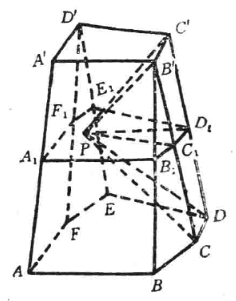
\includegraphics[scale=.7]{fig/2-102.png}
    \caption{}
\end{figure}


可以把这些棱锥分成两类：一类是以拟棱柱体的底面为底的，一类是以拟柱体的侧面为底的。

如图2.102，第一类的棱锥是$P-AC$和 $P-A' C'$, 它们的体积分别是：
\[\begin{split}
V_{P-AC}&=\frac{1}{3}S\cdot \frac{1}{2}h=\frac{1}{6}hS\\
V_{P-A'C'} &=\frac{1}{3}S' \cdot \frac{1}{2}h=\frac{1}{6}hS'     
\end{split}\]


第二类棱锥中，底面最多有三种情形：三角形、梯形和平行四边形.我们以其中一个，如棱锥 $P-CC'$ 为例看如何求它们的体积.

$\because\quad  C_{1}D_{1}$ 是中截面与侧面 $CC'$  的交线，

$\therefore\quad   C_{1}D_{1}$ 是梯形（或平行四边形） $B' CDC'$  的中位线，连结 $B' D_{1}$. 则
\[
S_{\text{梯形} B'CDC'} =4S_{\triangle C_{1}D_{1}B'}
\]

$\therefore\quad V_{P-CC' }=4V_{P-C_{1}D_{1}B'}$.

另一方面，
\[\begin{split}
V_{P-C_{1}D_{1}B'} &=V_{B'-PC_{1}D_{1}}\\
&=\frac{1}{3}\cdot \frac{h}{2}\cdot  S_{\triangle  PC_{1}D_{1}}\\
&=\frac{1}{6}hS_{\triangle  PC_{1}D_{1}}   
\end{split}\]

$\therefore\quad V_{P-CC' }=\frac{1}{6}h\cdot  4S_{\triangle PC_1D_1}$.

同样可以证明：
\[V_{P-DD'}=\frac{1}{6}h\cdot  4S_{\triangle PD_{1}E_{1}}, \ldots\]

把第二类棱锥的体积相加，得
\[
\frac{1}{6}h\left(4S{\triangle PC_{1}D_{1}}+4S{\triangle PD_{1}E_{1}}+\cdots \right)=\frac{1}{6}h\cdot  4S_{0}\]
\[\begin{split}
V_{\text{拟柱体 }}&=\frac{1}{6}hS+\frac{1}{6}h\cdot  4S_{0}+\frac{1}{6}hS' \\
&=\frac{1}{6}h\left(S+4S_{0}+S'\right)    
\end{split}\]

\begin{example}
    要筑一道大坝，下底面是长为580m、宽46m的矩形，上底面是长500m，宽14m的矩形，高23m，问共需料多少立方米？
\end{example}

\begin{analyze}
    这大坝的几何形状是拟柱体，只要求出它的上、下底面和中截面的面积及它的高.
\end{analyze}

\begin{solution}
这大坝是拟柱体，其中截面是矩形。
\[\begin{split}
\text{矩形长边}&=\frac{1}{2}(580+500)=540(\mathrm{m}),
\\
\text{矩形宽为}&=\frac{1}{2}(46+14)=30(\mathrm{m}),    
\end{split}\]

设上、下底面及中截面面积分别是$Q_{2}$, $Q_{1}$, $Q_{0}$, 则
\[\begin{split}
Q{1}&=580\x 46=26680\left(\mathrm{m}^{2}\right),
\\
Q{2}&=500\x 34=17000\left(\mathrm{m}^{2}\right),
\\
Q{0}&=540\x 30=16200\left(\mathrm{m}^{2}\right).    
\end{split}\]

\[\begin{split}
\therefore\quad V_{\text{拟柱体 }}&=\frac{1}{6}\cdot  h\left(Q_{1}+4Q_{0}+Q_{2}\right)    \\
&=\frac{1}{6}\x 23(26680+17000+4× 16200)\\
&=415840\left(\mathrm{m}^{3}\right).
\end{split}\]
答：筑此大坝共需料415840立方米。
\end{solution}


\subsection*{2.11 练习}
\begin{enumerate}
    \item 画一不是棱锥的拟柱体，使它的各面都是三角形。
    \item 举例说明，长方台$ABCD-A_{1}B_{1}C_{1}D_{1}$ 中， $A_{1}A$ 和 $CC_{1}$ 有可能是异面直线.
\item 说明 $V_{\text{棱柱 }}=Sh$, $V_{\text{棱锥 }}=\frac{1}{3}Sh$, $
V_{\text{棱台 }}=\frac{1}{3}h\left(S +\sqrt{SS'}+S'\right)$
是公式$V_{\text{拟柱体 }}=\frac{1}{6}h\left(S+4S_{0}+S' \right)$ 的特殊形式.

\noindent
\begin{minipage}{.45\textwidth}
\centering
\begin{tikzpicture}[scale=.8]
    \tkzDefPoints{0/0/A, 4/0/B, 5/1/C, 1/2/A_1, 3.5/2/B_1, 4.2/2.75/C_1}
\tkzDefPointsBy[translation=from B to C](A){D}
\tkzDefPointsBy[translation=from B_1 to C_1](A_1){D_1}


\tkzDrawPolygon(A,B,C,C_1,D_1,A_1)
\tkzDrawSegments[dashed](A,D C,D D,D_1)
\tkzDrawSegments[](A_1,B_1 B_1,C_1 B,B_1)
\tkzLabelPoints[left](A,A_1)
\tkzLabelPoints[right](B,C,B_1)
\tkzLabelPoints[above](D_1,C_1)
\tkzLabelPoints[below](D)
\end{tikzpicture}
\captionof*{figure}{（第2题）}
\end{minipage}\hfill
\begin{minipage}{.45\textwidth}
\centering
\begin{tikzpicture}
\tkzDefPoints{0/0/A, 1.2/1.5/B, .5/2.5/C, 4/0/A'}
\tkzDefPointsBy[translation=from A to A'](B,C){B',C'}

\tkzDrawPolygon(A,A',B',C',C)
\tkzDrawSegments[dashed](C,B B,B' A,B)
\tkzDrawSegments[](A',C')
\tkzLabelPoints[left](A,C)
\tkzLabelPoints[right](A',B',C')
\tkzLabelPoints[below](B)
\end{tikzpicture}
\captionof*{figure}{（第4题）}
\end{minipage}









\item 三棱柱$ABC-A' B' C'$  可以看作拟柱体的楔体$CC' -  AA' B' B$. 设$S_{AA' B' B}=S$, $CC'$  与平面$AA' B' B$ 的距离是$h$，用拟柱体公式求它的体积。

\item 
说明圆柱、圆锥、圆台的体积公式也可以写成
\[
V=\frac{1}{6}h\left(S+4S_{0}+S' \right).\]
其中，$h$是它们的高， $S'$、 $S$分别是上、下底的面积. $S_{0}$ 是中截面的面积。
\end{enumerate}



\section{球的体积公式}

当球的半径确定以后，球的大小就确定了.因此，球的体积是它的半径的函数.如何用球的半径表示它的体积呢？

以往我们每遇到一种几何体的体积计算问题，总是把新几何体转化为已学过的简单的几何体的体积计算问题.转化的方法有两种：一是把新几何体分割成我们会求其体积的几何体，一是利用祖暅原理。

虽然球面不能分割成平面，球也不能分割成柱锥台，但是我们可以用球的外切$n$面体的体积近似表示球的体积. 将球心与球外切$n$面体的各个顶点分别连结，则这个多面体可分割成$n$个棱锥，并且这$n$个棱锥的顶点都是球心，它们的高都是球的半径$R$，多面体的每一个面分别是棱锥的底面，设它们的面积分别是$S_{1},  S_{2},  S_{3},\ldots,  S_{n}$. 则
\[\begin{split}
 V_{\text{球外切$n$面体}}&=V_{1}+V_{2}+V_{3}+\ldots+V_{n}\\
&=\frac{1}{3}R\left(S_{1}+S_{2}+S_{3}+\cdots+S_{n}\right)   
\end{split}\]


当球外切$n$面体的面数$n$无限增大，并且$S_{1},  S_{2},  S_{3},\ldots, S_{n}$中最大的趋于零，则$S_{1}+S_{2}+S_{3}+\ldots+S_{n}$无限逼近球表面积$4\pi R^{2}$, 这样$V_{\text{球外切$n$面体 }}$的值无限逼近$\frac{1}{3}R\cdot 4\pi R^{2}$，即$\frac{4}{3}\pi R^{3}$. 这 
个值就应该是球的体积.

如何利用祖暅原理来推导半径为$R$的球体积公式？下面我们换一个思路讨论.

为了满足祖暅原理要求的条件，我们需找一个几何体，它要满足三个条件：
\begin{enumerate}[(1)]
    \item 它的“底”和半球的底面圆有相同的面积.
    \item 它的“高”应是$R$.
\item 把它和半球放在平面$\alpha$上后，用平行于$\alpha$的任意平面所截，截得的两个截面面积总应相等。
\end{enumerate}

这个几何体应是什么形状呢？我们进一步分析一下.

设截面和平面$\alpha$的距离是$L$，则截半球所得截面的面积是$\pi\left(R^{2}-L^{2}\right)$.

而$\pi \left(R^{2}-L^{2}\right)=\pi R^{2}-\pi  L^{2}$.

\begin{figure}[htp]
    \centering
\begin{tikzpicture}[scale=.7, very thick]
    \begin{scope}
\draw(-3,0) arc [start angle =180, end angle =0, radius=3];
\draw(-3,0) arc [start angle =180, end angle =360, x radius=3, y radius=.8];
\draw[dashed](-3,0) arc [start angle =180, end angle =0, x radius=3, y radius=.8];
\draw(150:3) arc [start angle =180, end angle =360, x radius=2.6, y radius=.5];
\draw[dashed](150:3) arc [start angle =180, end angle =0, x radius=2.6, y radius=.5];
\fill[pattern=north east lines] (0,1.5) ellipse [x radius=2.6, y radius=.5];

    \node at (0,-1.5){甲};
\end{scope}
\begin{scope}[xshift=8cm]
    \draw[pattern=north east lines](0,0) ellipse[x radius = 2.5, y radius=0.8];
    \draw[fill=white](0,0) ellipse[x radius = 1, y radius=0.25];
    \node at (0,-1.5){乙};
\end{scope}
\end{tikzpicture}

    \caption{}
\end{figure}


等式右端表示的是一个圆环的面积. 它的外圆半径是$R$，且不论截面在什么高度，它总是不变；它的内圆半径是$L$，它就是截面与平面$\alpha$的距离，所以它随截面与$\alpha$的距离加大而增大。

由此看来，我们需要的几何体具有这种性质：它的底面是半径为$R$的圆；当被平行于底面的平面截割后，截面是一圆环：圆环外圆与截面的高度无关，内圆的半径由$0\to R$.

因此，这个几何体就是从一个底面半径为$R$，高也是$R$
的一个圆柱，挖去一个以圆柱的上底面为底面，以圆柱的下底面圆心为顶点的圆锥，所剩余的部分。

从以上分析可以得到计算球的体积的方法：

取一个底面半径和高都等于$R$的圆柱，从圆柱中挖去一个圆锥，这个圆锥的底面是圆柱的上底面，这个圆锥的顶点是圆柱的下底面的圆心，把所得的几何体和半球放在同一平面$\alpha$上（图2.104），因为圆柱的高等于$R$，所以这个几何体和半球可以夹在两个平行平面之间。

\begin{figure}[htp]
    \centering
\begin{tikzpicture}[>=stealth]
\tkzDefPoints{0.5/0/a, 10.5/0/b, 12.5/2.5/c}
\tkzDefPointsBy[translation=from b to c](a){d}

\def\x{1.75}

\node at (12,2.25){$\alpha$};

\draw(2,1) arc (180:0:\x); 
\draw[dashed](2,1) arc [start angle=180, end angle =0, x radius=\x, y radius=0.4];
\draw[](2,1) arc [start angle=180, end angle =360, x radius=\x, y radius=0.4];
\draw[dashed](2,1)--(2+3.5,1);
\draw[dashed](2+\x,1)node[below]{$O$}--+(0,\x);
\draw[dashed](2+\x,1)--node[right]{$R$}++(30:\x)--++(-\x*0.5*1.732,0);
\node at (2+\x,1+\x*.25)[left]{$\ell$};
\fill[pattern= north east lines](2+\x,1+\x*.5) ellipse[x radius = \x/2*1.732, y radius = 0.35];
\tkzDefPoints{2+\x/1/O, 2+\x+\x*0.5*1.732/1+\x*.5/N'}
\draw(N') arc [start angle=0, end angle =-180, x radius = \x/2*1.732, y radius = 0.35];
\draw[dashed](N') arc [start angle=0, end angle =180, x radius = \x/2*1.732, y radius = 0.35];


\draw[dashed](7,1) arc [start angle=180, end angle =0, x radius=\x, y radius=0.4];
\draw[](7,1) arc [start angle=180, end angle =360, x radius=\x, y radius=0.4];

\draw[dashed](7,1+\x*.5) arc [start angle=180, end angle =0, x radius=\x, y radius=0.4];
\draw[](7,1+\x*.5) arc [start angle=180, end angle =360, x radius=\x, y radius=0.4];


\fill[pattern  = north east lines](7+\x,1+\x*.5) ellipse [x radius = \x, y radius = 0.4];
\draw[dashed, fill=white](7+\x,1+\x*.5) ellipse [x radius = .5*\x, y radius = 0.2];
\draw[<->](7+\x,0.5*\x+1)node[left]{$O_1$}--node{$\ell$}(7+1.5*\x,0.5*\x+1)node[right]{$B$};

\node[left] at (7,0.5*\x+1){$K$};
\node[right] at (7+2*\x,0.5*\x+1){$N$};

\tkzDefPoints{7+\x/1/O', 7+\x/1+\x*.5/N}

\draw[](7+\x, \x+1) ellipse [x radius=\x, y radius=0.4];

\draw[](7, 1)--+(0,\x)node[above left]{$L$};
\draw[](7+2*\x, 1)--+(0,\x)node[above right]{$P$};
\draw[dashed](7+2*\x, \x+1)--(2+\x,\x+1);
\draw[dashed](7+2*\x, \x+1)--(7+\x,1)node[below]{$O'$}--(7, \x+1);
\draw[dashed](7+2*\x, 1)--(7,1);
\draw[dashed](7+\x, 1)--+(0,\x);



\tkzDefPoints{2+\x/1/O, 2+2*\x/1/R', 7/1/L', 7+2*\x/1/P', 7/1+\x/L, 7+2*\x/1+\x/P}
\tkzInterLC[](c,d)(O,R')
\tkzGetPoints{tmp1}{tmp2}
\tkzInterLL(L,L')(c,d) \tkzGetPoint{tmp3}
\tkzInterLL(P,P')(c,d) \tkzGetPoint{tmp4}

\tkzDrawSegments(a,b b,c d,a c,tmp4 tmp2,d tmp1,tmp3)





\end{tikzpicture}
    \caption{}
\end{figure}

用平行于平面$\alpha$的任意一个平面去截这两个几何体，截面分别是圆面和圆环面，当截面与$\alpha$的距离为$\ell$时，圆面半径 $r=\sqrt{R^{2}-\ell^{2}}$，圆的大圆半径为$R$，小圆半径为$\ell$（因为 $O'O_{1}=O_{1}B$）.

$\because\quad S_{\text{圆}}=\pi r^{2}=\pi \left(R^{2}-\ell^{2}\right),\quad 
S_{\text{圆环 }}=\pi  R^{2}-\pi \ell^{2}=\pi \left(R^{2}-\ell^{2}\right)$,

$\therefore\quad  S_{\text{圆}}=S_{\text{圆环}}$

根据祖暅原理，这两个几何体的体积相等，即
\[
\frac{1}{2}V_{\text{球} }=\pi R^{2}\cdot  R-\frac{1}{3}\pi R^{2}\cdot  R=\frac{2}{3}\pi R^{2}\]

$\therefore\quad V_{\text{球 }}=\frac{4}{3}\pi R^{3}$

由此我们得到下述定理：
\begin{thm}
{定理} 如果球的半径是$R$，那么它的体积是
\[V_{\text{球 }}=\frac{4}{3}\pi R^{3}\]    
\end{thm}


这个公式还可以写成
\[
V_{\text{球}}=\frac{4}{3}\pi  R^{3}=\frac{1}{3}\left(4\pi R^{2}\right)R=\frac{1}{3}S_{\text{球面 }}\cdot  R\]
这就是说，球的体积可以看做一个锥体的体积，这个锥体的底面面积是球的表面积，而它的高是球的半径.

\begin{example}
    将直径为25cm及35cm的两个铸铁球，熔成一个球，求这球的直径。
\end{example}

\begin{analyze}
    这实质上是已知球的体积求其直径的问题.
\end{analyze}

\begin{solution}
$\because\quad V_{\text{球} }=\frac{4}{3}\pi R^{3}=\frac{4}{3}\pi \left(\frac{d}{2}\right)^{3}=\frac{\pi }{6}d^{3}$，设所求直径为$x$,

$\therefore\quad \frac{\pi 25^{3}}{6}+\frac{\pi 35^{3}}{6}=\frac{\pi x^{3}}{6}$,

\[x^{3}=25^{3}+35^{3}\]

$\therefore\quad x\approx 39$.

答：熔成后的那球的直径约为39cm.
\end{solution}

\begin{example}
    一个倒圆锥形的漏斗，底面半径为$a$，母线的长是 $b,\quad (b>a)$，把一个球放在这漏斗内，漏斗的底面正好和球相切，求这球的体积.
\end{example}

\begin{analyze}
欲求这球的体积，只要求出它的半径. 这就要通过圆锥的轴截面来解决. 因为轴截面总是包含了已知量和未知量的平面图形. 这就把立体问题转化为平面问题.
\end{analyze}

\begin{figure}[htp]
    \centering
\begin{tikzpicture}
\begin{scope}
    \tkzDefPoints{-1.5/3/A, 1.5/3/B, 0/0/S, 0/3/M}

\tkzDefTriangleCenter[in](B,S,A)
\tkzGetPoint{O}
\tkzDrawCircle[dashed](O,M);
\tkzInterLC(A,S)(O,M)
\tkzGetPoints{C}{C2}
\tkzDrawSegments(S,A B,S)
\draw(M) ellipse [x radius = 1.5, y radius=.5];
\draw[dashed](C) arc [start angle =180, end angle=0, x radius=.8, y radius=.25];
\tkzDrawPoints(O,M)
\draw(C) arc [start angle =180, end angle=360, x radius=.8, y radius=.25];

\tkzLabelPoints[above](M)
\tkzLabelPoints[below](S)
\tkzLabelPoints[left](A)
\tkzLabelPoints[right](O,B)
\tkzDrawSegments[dashed](S,M)
\node at (0,-1){(甲)};
\end{scope}
\begin{scope}[xshift=6cm]
    \tkzDefPoints{-1.5/3/A, 1.5/3/B, 0/0/S, 0/3/M}
\tkzDrawPolygon(A,B,S)
\tkzDefTriangleCenter[in](B,S,A)
\tkzGetPoint{O}
\tkzDrawCircle(O,M);
\tkzInterLC(A,S)(O,M)
\tkzGetPoints{C}{C2}

\tkzLabelPoints[above](A,M,B)
\tkzLabelPoints[below](S)
\tkzLabelPoints[left](C)
\tkzLabelPoints[right](O)
\tkzDrawSegments[dashed](S,M)
\node at (0,-1){(乙)};
\tkzDrawSegments(O,C)

\end{scope}
\end{tikzpicture}
    \caption{}
\end{figure}


\begin{solution}
作轴截面如图， $AM=a$,  $SA=b$,  $OM=OC=R$,

在${\rm Rt}\triangle AMS$中， $MS=\sqrt{b^{2}-a^{2}}$, $OS=\sqrt{b^{2}-a^{2}}-R$,

又$\triangle SMA\backsim \triangle  SCO$,  

$\therefore\quad \frac{SO}{SA}=\frac{OC}{AM}$.

即$\frac{\sqrt{b^{2}-a^{2}}-R}{b}=\frac{R}{a}$,  

$\therefore\quad R=\frac{c\sqrt{b^{2}-a^{2}}}{a+b}$

$\therefore\quad V_{\text{球} }=\frac{4}{3}\pi \frac{a^{3}\left(b^{2}-a^{2}\right)\sqrt{b^{2}-a^{2}}}{(a+b)^{3}}
=\frac{4\pi a^{3}(b-a)\sqrt{b^{2}-a^{2}}}{3(a+b)^{2}}$.
\end{solution}





\subsection*{2.12 练习}

一、填空题：
\begin{enumerate}
    \item 如果一个球的半径扩为原来的3倍，则这球的体积扩大为原来的$\underline{\qquad\qquad}$倍.

    \item 火星的直径是地球直径的一半，则火星体积是地球体积
的$\underline{\qquad\qquad}$倍。

\item 木星的面积约是地球面积的120倍，它的体积约是地球体积的$\underline{\qquad\qquad}$倍。
\item 
铜球由于加热膨胀而使半径增加$\frac{1}{1000}$，那么它的体积增加$\underline{\qquad\qquad}$.

\item 一个正方体的顶点都在球面上，它的棱长是4cm，那么这球的体积是$\underline{\qquad\qquad}$.
\item 
正三棱柱的内切球半径是$R$，则正三棱柱的体积是$\underline{\qquad\qquad}$.
\item 
一个棱长为4的正方体，其外接球的体积是$\underline{\qquad\qquad}$.

\item 圆锥的底面半径是$r$，高为$h$，它的内切球的半径是$\underline{\qquad\qquad}$.
\item 
正四棱锥的棱长为$a$，它的外接球的半径是$\underline{\qquad\qquad}$.
\item 
正三棱锥的各棱长都是$a$，则它的内切球的半径是$\underline{\qquad\qquad}$，外接球的半径是$\underline{\qquad\qquad}$.
\item 
三个球的半径的比是1:2:3，那么最大球的体积是其余两个球的体积和的$\underline{\qquad\qquad}$倍。
\end{enumerate}


二、选择题：
\begin{enumerate}
    \item 等边圆锥和它的内切球的体积之比为 \hfill (\qquad )
\begin{multicols}{4}
\begin{enumerate}[(A)]
    \item 9:4
    \item 9:5
    \item 3:2
    \item 12:5
\end{enumerate}
\end{multicols}

\item 球的体积与这球的外切圆柱的体积和这球的外切等边圆锥的体积之比为\hfill (\qquad )
\begin{multicols}{4}
\begin{enumerate}[(A)]
    \item 1:2:3
    \item 2:3:6
    \item 4:6:9
    \item 1:2:4
\end{enumerate}
\end{multicols}

\item 等体积的球与等边圆柱的表面积分别是$S_{1}$, $S_{2}$，则$S_{1}:S_{2}$ 等于\hfill (\qquad )
\begin{multicols}{2}
\begin{enumerate}[(A)]
    \item $\sqrt[3]{\frac{2}{3}}$
    \item $\sqrt{\frac{2}{3}}$
    \item $\frac{2}{3}$
    \item 不同于上述的其它答案
\end{enumerate}
\end{multicols}

\item 等体积的球与正方体表面积的大小关系是 \hfill (\qquad )
\begin{multicols}{2}
\begin{enumerate}[(A)]
    \item $S_{\text{球 }}=S_{\text{正方体 }}$
    \item $S_{\text{球 }}>S_{\text{正方体 }}$
    \item $S_{\text{球 }}<S_{\text{正方体 }}$
    \item 不能确定
\end{enumerate}
\end{multicols}


\item 球面上有三点$A$、$B$、$C$，若 $AB=18$,  $BC=24$,  $AC= 80$，且球心到$\triangle ABC$所在平面的距离是球半径的 $\frac{1}{2}$，则球的半径$R$等于\hfill (\qquad )
\begin{multicols}{4}
\begin{enumerate}[(A)]
    \item $\frac{10}{\sqrt{3}}$
    \item 10
    \item $10\sqrt{3}$
    \item $\frac{20}{\sqrt{3}}$
\end{enumerate}
\end{multicols}


\item 如果一个圆柱和一个圆锥的底面直径和高都与球的直径相等，那么圆柱、球、圆锥体积的比是 \hfill (\qquad )
\begin{multicols}{4}
\begin{enumerate}[(A)]
    \item 24:32:8
    \item 3:2:1
    \item 6:3:2
    \item 9:6:4
\end{enumerate}
\end{multicols}


\item 一个球的内接正方体体积是8，则此球的体积是\hfill (\qquad )
\begin{multicols}{4}
\begin{enumerate}[(A)]
    \item $\frac{2\sqrt{3}}{3}\pi$
    \item $4\sqrt{3}\pi$
    \item $\frac{2\sqrt{6}}{3}\pi$
    \item $4(\sqrt{3}+1)\pi $
\end{enumerate}
\end{multicols}


\item 三个球的表面积之比是1:2:3，则它们的体积比是\hfill 
(\qquad )
\begin{multicols}{2}
\begin{enumerate}[(A)]
    \item 1:4:9
    \item $1:\sqrt{2}:\sqrt{3}$
    \item 1:2:3
    \item $1:2\sqrt{2}:3\sqrt{3}$
\end{enumerate}
\end{multicols}
\end{enumerate}

\section{球缺和球缺的体积公式}

固定钢板用的圆头铆钉的圆头具有球缺的形象。一个球被平面截下的一部分叫做球缺，截面叫做球缺的底面，垂直于截面的直径被截下的线段长叫做球缺的高.



球缺是旋转体，它可由弓形绕着与弓形的弦垂直的直径旋转而得到. 球缺也可以看做是球冠和球冠的底所在的圆面所围成的几何体.

\begin{figure}[htp]
    \centering
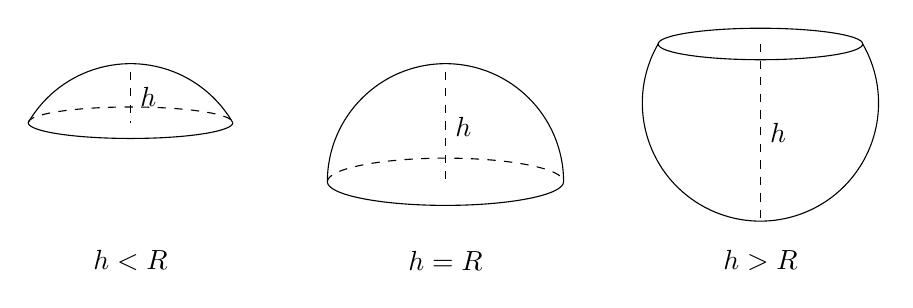
\begin{tikzpicture}[scale=.5]
\begin{scope}
\draw(150:3) arc (150:30:3);
\draw[dashed](150:3) arc [start angle =180, end angle =0, x radius = 1.5*1.732, y radius = .4];
\draw(150:3) arc [start angle =180, end angle =360, x radius = 1.5*1.732, y radius = .4];
\draw[dashed](0,2.8)--node[right]{$h$}(0,1.5);
\node at (0,-2){$h<R$};

\end{scope}
\begin{scope}[xshift=8cm]
    \draw(180:3) arc (180:0:3);
\draw[dashed](180:3) arc [start angle =180, end angle =0, x radius = 3, y radius = .6];
\draw(180:3) arc [start angle =180, end angle =360, x radius = 3, y radius = .6];
\draw[dashed](0,2.8)--node[right]{$h$}(0,0);
\node at (0,-2){$h=R$};

\end{scope}


\begin{scope}[xshift=16cm, yshift=2cm]
    \draw(150:3) arc (150:390:3);
\draw(150:3) arc [start angle =180, end angle =0, x radius = 1.5*1.732, y radius = .4];
\draw(150:3) arc [start angle =180, end angle =360, x radius = 1.5*1.732, y radius = .4];
\draw[dashed](0,1.5)--node[right]{$h$}(0,-3);
\node at (0,-4){$h>R$};

\end{scope}
\end{tikzpicture}
    \caption{}
\end{figure}



我们在推导球的体积公式时，是先推导出一个特殊球缺——半球的体积，再2倍后得到的. 对于一般的球缺，即$h \ne R$ 时，它的体积公式的推导方法完全类似，只不过是把球的高$R$用一般球缺的高$h$去代替，如图2.106。所以当球的半径为$R$，球缺的高为$h$时，有
\[\begin{split}
    V_{\text{球缺 }}&=V_{\text{圆柱} LKNP}-V_{\text{圆台} LABP}\\
    &=\pi  R^{2}h-\frac{1}{3}\pi  h\left[R^{2}+R(R-h)+(R-h)^{2}\right]\\
    &=\pi  R^{2}h-\pi  R^{2}h+\frac{1}{3}\left(3\pi  Rh^{2}\right)-\frac{1}{3}\pi  h^{3}\\
    & =\frac{1}{3}\pi  h^{2}(3R-h).
\end{split}\]

若球缺的高 $h' =2R-h$,

$\because\quad  h<R,\qquad   \therefore h' >R$. 这时
\[\begin{split}
    V_{\text{大球缺 }}&=V_{\text{球 }}-V_{\text{小球缺 }}\\
&=\frac{4}{3}\pi  R^{3}-\frac{1}{3}\pi  h^{2}(3R-h)\\
&=\frac{1}{3}\pi \left(4R^{3}-3Rh^{2}+h^{3}\right)
\end{split}\]
而把公式 $\frac{1}{3}\pi  h^{2}(3R-h)$ 中的$h$换作$h' =2R-h$ 则得
\[\begin{split}
\frac{1}{3}\pi \left(2R-h^{2}\right)[3R-(2R-h)]&
=\frac{1}{3}\pi \left(4R^{2}-4Rh+h^{2}\right)(R+h)
\\
&=\frac{1}{3}\pi \left(4R^{3}-3R^{2}h+h^{3}\right)    
\end{split}\]

$\therefore\quad$ 当球缺的高$h' >R$ 时
仍有
\[V_{\text{球缺 }}=\frac{1}{3}\pi  h^{\prime 2}\left(3R-h' \right)\]

$\therefore\quad$ 我们有下面的定理：

\begin{thm}
{定理} 如果球的半径是$R$，球缺的高是$h$，那么球缺的体积是
\[V_{\text{球缺 }}=\frac{1}{3}\pi  h^2 \left(3R-h \right)\]
\end{thm}

\begin{example}
 一扇形的半径是$R$，中心角是$60^{\circ}$，绕着它的半径旋转一周，求旋转体的体积.
\end{example}

\noindent
\begin{minipage}{.5\textwidth}\CTEXindent
\begin{analyze}
这个旋转体可分为一个球缺和一个圆锥，如图2.107. 

设球缺的高是$h$，则
\[
h=R-R\cdot \cos 60^{\circ}=R-\frac{R}{2}=\frac{R}{2}\]
从而可求得球缺的体积.

圆锥的高和底面半径$r$可通过它的母线长（等于$R$）和 $60^{\circ}$ 的中心角求出. 故其体积可求.
\end{analyze}
\end{minipage}\hfill
\begin{minipage}{.46\textwidth}
\centering
\begin{tikzpicture}[scale=.9]
\tkzDefPoints{0/0/O, 0/1.5/C, 2.6/1.5/B, -2.6/1.5/A, 0/3/D}
\draw(A) arc [start angle = 180, end angle=360, x radius = 2.6, y radius=.4];
\draw[dashed](A) arc [start angle = 180, end angle=0, x radius = 2.6, y radius=.4];
\tkzDrawSegments[dashed](C,O)
\tkzDrawSegments(A,O)
\draw(A) arc (150:30:3);
\tkzLabelPoints[left](A,C)
\tkzLabelPoints[right](B)
\tkzLabelPoints[above](D)
\tkzLabelPoints[below](O)
\draw[dashed](C)--node[above]{$r$}(B);
\draw[dashed](C)--node[right]{$h$}(D);
\draw[](O)--node[below]{$R$}(B);
\node at (60:.7){$60^{\circ}$};



\end{tikzpicture}
\captionof{figure}{}
\end{minipage}



\begin{solution}
\[V_{\text{球缺 }}=\frac{1}{3}\pi \left(\frac{R}{2}\right)^{2}\left(3R-\frac{R}{2}\right)=\frac{5}{24}\pi  R^{3}\]

圆锥的高是 $R\cdot \cos 60^{\circ}=\frac{R}{2}$,

底面半径是 $R\cdot \sin60^{\circ}=\frac{3}{2}R$,

$\therefore\quad V_{\text{圆锥}}=\frac{1}{3}\pi \left(\frac{\sqrt{3}}{2}R\right)^{2}\cdot \frac{R}{2}=\frac{\pi }{8}R^{3}$.

$\therefore\quad$ 所求旋转体的体积是
\[V=V_{\text{球缺 }}+V_{\text{圆锥}}=\frac{5}{24}\pi  R^{3}+\frac{\pi }{8}R^{3}=\frac{1}{3}\pi  R^{3}.\]
\end{solution}


\begin{thm}
    {思考题：}
将例2.48的结果变形，得
\[V=\frac{1}{3}R\cdot (\pi R^2)=\frac{1}{3}R\left(2\pi R\cdot \frac{R}{2}\right)=\frac{1}{3}R\cdot S_{\text{球冠}}\]
你对它可作何解释？
\end{thm}

\begin{example}
    已知：球缺底面半径是$r$，高是$h$. 求证：球缺的体积是
\[V_{\text{球缺 }}=\frac{1}{6}\pi  h\left(3r^{2}+h^{2}\right).\]
\end{example}

\begin{proof}
    
\end{proof}


设截得球缺的球的半径是$R$，作轴截面如图2.108.

\begin{figure}[htp]
    \centering
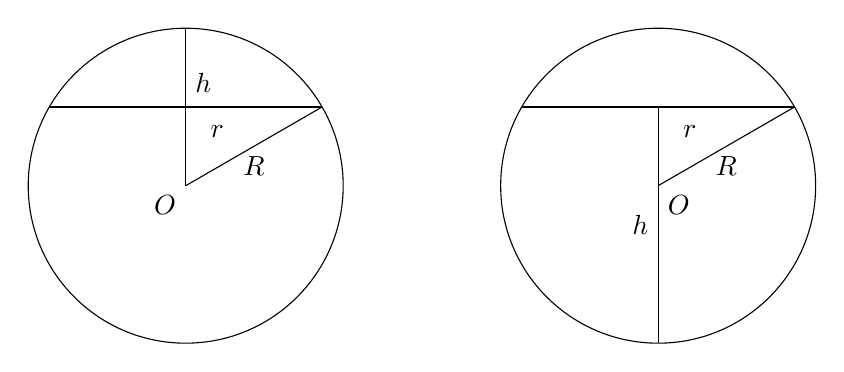
\begin{tikzpicture}
\begin{scope}
\draw(0,0)node[below left]{$O$} circle (2);
\draw(30:2)--(150:2);
\node at (60:.8){$r$};
\draw(0,0)--(0,2);
\node at (0,1.3)[right]{$h$};
\draw(0,0)--node[below]{$R$}(30:2);
\end{scope}
\begin{scope}[xshift=6cm]
    \draw(0,0)node[below right]{$O$} circle (2);
\draw(30:2)--(150:2);
\node at (60:.8){$r$};
\draw(0,1)--node[left]{$h$}(0,-2);
\draw(0,0)--node[below]{$R$}(30:2);
\end{scope}
\end{tikzpicture}
    \caption{}
\end{figure}

设球缺的高为$h$.

则$r^{2}=R^{2}-(R-h)^{2}
=2Rh-h^{2}$,

$\therefore\quad R=\frac{r^{2}}{2h}+\frac{h}{2}$.

代入球缺体积公式，得
\[\begin{split}
V_{\text{球缺 }}&=\pi  h^{2}\left(R-\frac{1}{3}h\right)\\
&=\pi  h^{2}\left(\frac{r^{2}}{2h}+\frac{h}{2}-\frac{h}{3}\right)\\
&=\frac{1}{6}\pi  h\left(3r^{2}+h^{2}\right).    
\end{split}\]

\begin{remark}
\begin{enumerate}
    \item 上式推导对$h<r$,  $h=r$ 和 $h>r$ 都成立.
    \item 球缺的体积公式对球的体积也适用.
    \item  在生产和生活中所遇到的物体，形状虽然比较复杂，但是很多都可以看作是由柱体、锥体、台体、球体、球快等组合（例如铆钉）或切割（例如螺帽）而成的，所以，我们能求这些几何体的体积，就能求那些形状比较复杂的物体的体积. 然而，还有一些物体的体积（例如抛物线绕其对称轴旋转所得旋转体的体积），要用高等数学中的积分法才能解决。
\end{enumerate}
\end{remark}





\subsection*{2.13 练习}
\begin{enumerate}
    \item 一个球缺的高是球的直径的$\frac{1}{10}$，求它们体积之比。
\item 
一个球缺的底面半径是球的半径的$\frac{1}{2}$，其体积是球的几分之几？

\begin{figure}[htp]
    \centering
\begin{tikzpicture}[>=stealth]
\begin{scope}
\draw(150:2)--(30:2);
\draw(150:2) arc (150:30:2);
\draw(-.8,-2) rectangle (.8, 1);
\draw[|<->|](-.8,-2.5)--node[fill=white]{22}(.8,-2.5);
\draw[dashdotted](0,-2.25)--(0,2.5);
\draw[|<->|](-1.732,2.5)--node[fill=white]{39}(1.732,2.5);
\draw(-1.732,2.75)--(-1.732,1);
\draw(1.732,2.75)--(1.732,1);
\draw[|<->|](-2.25,2)--node[fill=white]{14}(-2.25,1);

\draw(-2.5,2)--(-1.732,2);
\draw(-2.5,1)--(-1.732,1);

\end{scope}
\begin{scope}[xshift=6cm]
    \draw(150:2)--(30:2);
\draw(150:2) arc (150:30:2);
\draw(-150:2)--(-30:2);
\draw(-150:2) arc (-150:-30:2);
\draw(-.8,-1) rectangle (.8,1);
\draw[dashdotted](0,-2.75)--(0,2.75);
\fill[pattern=north east lines](-.8,-1) rectangle(-2.5,0);
\fill[pattern=north east lines](.8,-1) rectangle(2.5,0);
\fill[pattern=north west lines](-.8,0) rectangle(-2.5,1);
\fill[pattern=north west lines](.8,0) rectangle(2.5,1);
\draw(-.8,0)--(-2.5,0)  (.8,0)--(2.5,0);
\draw(-2.5,1)--(2.5,1)  (-2.5,-1)--(2.5,-1);
\end{scope}

    
\end{tikzpicture}
    \captionof*{figure}{（第3题）}
\end{figure}

\item 长江大桥的钢梁结构是用铆钉铆合的（如图，单位：mm）。铆钉头是球缺形，钉身是圆柱形，铆钉插入两块钢板铆合后，两侧钉头大小
相等，已知每块钢板厚12mm，求钉身长度。
\end{enumerate}


\section*{习题七}
\begin{center}
    \bfseries A
\end{center}

\begin{enumerate}
    \item 一个体积为$48\sqrt{3}\mathrm{cm}^{3}$ 的正三棱柱有内切球，求这球的体积.

    \item 一个平面分球面为1:2两部分，求这个平面把球分成的两个球缺的体积的比.
    \item 
圆台的上、下底面半径分别是$r$和$R$，求它的内切球的半径.
    \item 
球的半径为3cm，在其正中钻一个半径为1cm的圆孔，求剩余部分的体积.
    \item 
一个木球浮于水中，在水面上的球缺高为2cm，底面半径为8cm，求这个木球的质量.（木球密度$0.8{\rm kg}/{\rm cm}^3$）
\end{enumerate}

\begin{center}
    \bfseries B
\end{center}

\begin{enumerate}
\setcounter{enumi}{5}   
 \item 在半径为a的半球形碗中盛满水，将碗口倾斜$30^{\circ}$, 求这时留在碗中的水的体积.
 \item 三棱锥$V-ABC$中， $VA\perp \text{底面} ABC$,  $\angle ABC=90^{\circ}$,  $VA=a$, $ BC=b$,  $AC=c\; (c>b)$. 
 
 求证：$V$、$A$、$B$、$C$四点在同一个球面上.
\end{enumerate}


\begin{center}
    \bfseries C
\end{center}

\begin{enumerate}
\setcounter{enumi}{7}
\item 若球的外切圆台的体积为球体积的三倍，求此圆台的母线和下底面所成的角$\alpha$之半的正切值 $\left(0^{\circ}<\alpha<90^{\circ}\right)$.
\end{enumerate}

\section{本章小结}
\subsection{知识结构分析}

\begin{landscape}
\subsection*{多面体}

\begin{tikzpicture}[>=stealth]
\node(A) at (-2,0){多面体};
\node(A1) at (0,0){凸多面体};
\node(B1) at (3,5){棱柱};
\node(B2) at (5,5){直棱柱};
\node(B3) at (8,6){正棱柱};
\node(B4) at (8,4){长方体};
\node(B5) at (11,4){正方体};
\draw[->](A)--(A1);  
\draw[->](A1)--(B1); 
\draw[->](B1)--(B2);  
\draw[->](B2)--(B3) ;
\draw[->](B2)--(B4) ;
\draw[->](B4)--(B5);
\draw[->](A1)--(B1);  
\draw[->](B1)--(B2);  




\node(C1) at (3,0){棱锥};
\node(C2) at (6,0){正棱锥};

\draw[->](A1)--(C1);  
\draw[->](C1)--(C2);  


\node(D1) at (3,-5){棱台};
\node(D2) at (6,-5){正棱台};
\draw[->](A1)--(D1);  
\draw[->](D1)--(D2);  


\node[draw](E1) at (5,6){棱柱的性质};
\draw[->](B1)--(E1);

\node[align=left, draw] (E2) at (5,2.5){直棱柱性质\\直观图画法\\侧面展开图\\侧面积、全面积};
\draw[->](B2)--(E2);

\node[draw](E3) at (9,2.5){对角线性质};
\draw[->](B4)--(E3);

\node[draw](F1) at (3,-1.5){棱锥的性质};
\draw[->](C1)--(F1);
\node[align=left, draw] (F2) at (10,0){正棱锥性质\\直观图画法\\侧面展开图\\侧面积、全面积};
\draw[->](C2)--(F2);

\node[draw](G1) at (4,-3.5){棱台的性质};
\draw[->](D1)--(G1);
\node[align=left, draw] (G2) at (10,-3){正棱台性质\\直观图画法\\侧面展开图\\侧面积、全面积};
\draw[->](D2)--(G2);
\end{tikzpicture}
\end{landscape}




\subsection*{旋转体}
\begin{tikzpicture}[>=stealth]
\node(A) at (-3,0){旋转体};
\node(A1) at (0,3){圆柱};
\node(B1) at (0,1.5){圆锥};
\node(B2) at (0,0){圆台};
\node(B3) at (0,-4){球和球面};
\node(B4) at (3,-4){球冠};

\draw[->](A)--(A1);
\draw[->](A)--(B1);
\draw[->](A)--(B2);
\draw[->](A)--(B3);
\draw[->](B3)--(B4);
\draw[->](B1)--(B2);


\node[align=left, draw] (C1) at (5,1.5){圆柱、圆锥、圆台的性质\\直观图的画法\\侧面展开图\\侧面积和全面积};
\draw[->](A1)--(C1);
\draw[->](B1)--(C1);
\draw[->](B2)--(C1);

\node[align=left, draw] (C2) at (3.5,-1.5){球的性质\\球的截面的性质\\直观图的画法\\表面积};
\draw[->](B3)--(C2);

\node[draw](C3) at (6,-4) {球冠的面积};
\draw[->](B4)--(C3);

\end{tikzpicture}







\begin{landscape}
\subsection*{体积概念及公理}
\begin{tikzpicture}[>=stealth]
    \node[align=left, draw] (A1) at (-2,0){体积概念\\体积公理};
    \node[align=left, draw] (A2) at (2,2){等底面积等高\\的两个锥体\\体积相等};
    \node[align=left, draw] (A3) at (2,-2){等底面积等高\\的两个柱体\\体积相等};
\draw[->](A1)--(A2);
\draw[->](A1)--(A3);

\node[align=center, draw](B1) at (7,2) {锥体\\体积公式};
\node[align=center, draw](B2) at (6,-2) {柱体\\体积公式};
\draw[->](A2)--(B1);
\draw[->](A3)--(B2);

\node[align=center, draw](C1) at (13,3.5) {拟柱体\\体积公式};
\node[align=center, draw](C2) at (13,0.5) {台体\\体积公式};
\draw[->](B1)--(C1);
\draw[->](B1)--(C2);
\draw[->](C1)--(C2);

\node[align=center, draw](D2) at (9,-3) {球的\\体积公式};
\node[align=center, draw](D1) at (13,-3) {球缺\\体积公式};

\draw[->](B2)--(D2);
\draw[->](B1)--(D2);
\draw[->](C2)--(D1);
\draw[->](B2)--(B1);
\draw[->](D1)--(D2);
\draw[->](C2)--(D2);




\end{tikzpicture}

\end{landscape}


\subsection{几点说明}

（1）通过对本章多面体和旋转体的性质的研究，我们对它们的认识就比较全面，比较深刻了.

一个几何图形（平面图形，或空间图形）的几何性质，主要是指它们的元素及某些位置的截面的形状、大小和位置关系. 我们所获得的一些结论都是在第一章关于直线和平面的基本理论的基础上推导出来的，即不是靠直接观察，也不是靠实验而是靠推理得到的.

这种从公理出发靠推理获得结论的一套方法，是我们学习几何这门课程的重要内容. 它对我们思维的逻辑性、严密性、准确性的培养和训练是其它学科难以代替的，如果这方面放松了要求，我们就没有达到学习立体几何的目的.

所以无论是证明题还是计算题，在作解答时，决不能靠直观和想当然来判断和叙述. 进行逻辑推理时要注意严密，不能马虎.

例如要判断直线$\ell$垂直平面$\alpha$，就要写出直线垂直平面的充分条件：
\begin{enumerate}
    \item 对任意的 $a \subset\alpha$, 都有$\ell\perp a$;

    \item $\ell\perp a$,  $\ell\perp b$,
$a\subset\alpha$, $b\subset\alpha$,$a\cap b=A$;

    \item $\ell\parallel a$,  $a\perp\alpha$;

    \item  $\ell\perp\beta$,  $\alpha \parallel \beta$;

    \item  $\alpha \perp\beta$,  $\alpha \cap\beta =a$,  $\ell\subset\beta$,  $\ell\perp a$;

    \item  $\beta \perp\alpha$,  $\gamma\perp\alpha$,  $\beta \cap \gamma =\ell$.
\end{enumerate}


注意，以上每一条都可单独使用，但每一条一定要把条件写全.


类似这方面的内容，在第一章中都总结过了，这里不再赘述，这里只是强调，对证明过程，叙述的要求不能比第一章低，不能因有计算内容而忽视推理.


（2）在复习时要注意概括，这样可以加深对几何图形性质的认识.

例如直棱柱、正棱锥、正棱台、正棱锥、圆柱、圆锥、圆台，所有这些几何体的侧面积都可用一个公式表示：
\[S_{\text{侧} }=C_{0}L\]
其中， $C_{0}$ 是中截面周长，$L$分别表示侧棱长，斜高或母线长.

又如球面、球冠、球带的面积都可用下述公式表示：
\[
S=2\pi  Rh=\text{球的大圆的周长}\x \text{高}\]
其中，$R$是球的半径，$h$是高或直径.

柱、锥、台的体积公式可用台的体积公式来概括.

\begin{center}
\begin{tikzpicture}[>=stealth]
    \node [draw](A) at (0,3){$V_{\text{台体 }}=\frac{1}{3}h\left(S+\sqrt{SS' }+S' \right)$};
\node[draw] (B1) at (-3,0){$V_{\text{柱体 }}=Sh$};
\node[draw] (B2) at (3,0){$V_{\text{锥体 }}=\frac{1}{3}Sh$};
\draw[->](A)--node[fill=white]{$S'=S$}(B1);
\draw[->](A)--node[fill=white]{$S'=0$}(B2);
\end{tikzpicture}
\end{center}

小于半球的球缺、半球、大于半球的球缺、球的体积都可用下述公式表示：
\[
V=\frac{1}{3}\pi  h^{2}(3R-h)\]
其中$R$是球的半径，$h$是高或直径.

可以验证，所有柱（棱柱、圆柱）、锥（棱锥、圆锥）、台（棱台、圆台）的体积公式，球和球缺的体积公式都可以写成拟柱体公式：
\[
V=\frac{1}{6}h\left(S+4S_{0}+S' \right)
\]
其中，$S$和$S'$  是上、下底面积，$S_{0}$是中截面面积，$h$是高（对球来说：$S' =S=0$,  $h=2R$）.

（3）本章内容所体现的几种转化方法

转化是解决数学问题经常使用的一种思想，把未知转化为已知，把难转化为易是转化的基本方向. 本章内容所涉及到的转化方法如下：

\subsection*{把立体问题转化为平面问题}

棱锥性质的证明，正棱锥性质中的两个直角三角形，正棱台性质中的两个直角梯形，旋转体中的轴截面等都是把立体问题转化为平面问题处理.

柱、锥、台的侧面积都是通过把侧面沿一条棱或一条母线剪开，把它展成平面图形的办法推导其侧面积公式的.

其中作轴截面的方法是必须掌握好的重点，尤其对旋转体与多面体的组合体，作出旋转体的轴截面时，多面体的截面成什么形状是需要认真考虑的. 例如：一正方体内接于一圆锥，这是一组合体. 当圆锥的轴截面过正方体的对角面时，形状如图2.109甲；当圆锥的轴截面平行于正方体的一个侧面时，则这组合体的截面图形如图2.109乙；当圆锥的轴截面不与正方体的任何面平行目不过正方体的对角面时，组合体的截面图如图2.109丙所示.

要画出正方体内接于圆锥的示意图，简便的方法仍是先画出圆锥的轴截面，步骤如下：
\begin{figure}[htp]
    \centering
\begin{tikzpicture}[scale=.85]
    
\begin{scope}
\tkzDefPoints{-2/0/A,2/0/B, 0/4/C}
\tkzDrawPolygon[](A,B,C)
\node at (0,-1){甲};
\def\x{1.67}
\draw(-\x*1.414/2,0) rectangle (\x*1.414/2,\x);
\node at (0,\x)[above]{$b=\sqrt{2}a$};
\node at (\x*1.414/2,\x/2)[right]{$a$};

\end{scope}
\begin{scope}[xshift=5cm]
    \tkzDefPoints{-2/0/A,2/0/B, 0/4/C}
\tkzDrawPolygon[](A,B,C)
\node at (0,-1){乙};
\def\x{1.67}
\draw(-\x/2,0) rectangle (\x/2,\x);
\node at (0,\x)[above]{$b=a$};
\node at (\x/2,\x/2)[right]{$a$};

\end{scope}
\begin{scope}[xshift=10cm]
    \tkzDefPoints{-2/0/A,2/0/B, 0/4/C}
\tkzDrawPolygon[](A,B,C)
\node at (0,-1){丙};
\def\x{1.67}
\draw(-\x*1.414/2+0.3,0) rectangle (\x*1.414/2-0.3,\x);
\node at (0,\x)[above]{$a<b<\sqrt{2}a$};
\node at (\x*1.414/2-.3,\x/2)[right]{$a$};
\end{scope}
\end{tikzpicture}
    \caption{}
\end{figure}

\begin{enumerate}[(a)]
    \item 画过正方体对角面的轴截面.

    \item 画圆锥底面——描圆，并在椭圆内画正方形的直观图.

    \item 画正方体的“侧棱”和“上底面”成图（图2.110）.
\end{enumerate}

\begin{figure}[htp]
    \centering
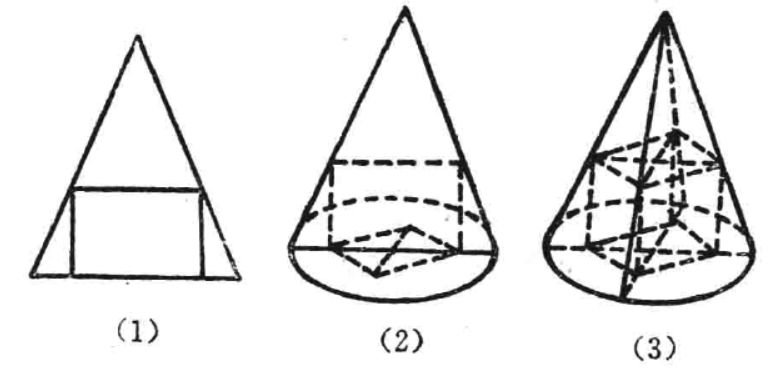
\includegraphics[scale=.4]{fig/2-110.png}
    \caption{}
\end{figure}




\subsection*{分割与组合的方法}

在推导三棱锥的体积公式时，是把一个三棱锥补成了三棱柱. 三棱锥的体积之所以是这三棱柱体积的 $\frac{1}{3}$，就是因为这三棱柱可以被分割成三个体积相等的三棱锥.

求拟柱体体积就纯粹用分割法，把拟柱体分割为两类三棱锥.

求球的体积和球缺的体积是找了一个组合体使这组合体的体积与半球或一般球缺的体积相等。

无论是分割，还是组合都是把要计算体积的几何体转化为我们已知其体积公式的几何体，这种思想方法必须掌握. 为了分割、组合的合理简便，我们对基本的几何体（会计算其体积的）必须熟悉其性质，同时要有一定的空间想象力和画图能力.

例如：斜三棱柱的一个侧面的面积为$S$，这个侧面与它所对的棱的距离等于$a$. 求证：这个棱柱的体积等于$\frac{1}{2}Sa$.

我们可以把这三棱柱看成拟柱体（面积为$S$的侧面作为拟柱体的底面，$a$就是这拟柱体的高），但是不用拟柱体的知识，用组合、分割的思想方法来处理这个问题，会很简捷.
\begin{enumerate}[(1)]
    \item  用组合的思想，把斜三棱柱 $ABC-A' B' C'$  补成一个四棱柱 $ADD' A' -CBB' C'$，就成了这棱柱的高.三棱柱$ ABC-A' B' C'  $的侧面$ BB' C' C $就成了四棱柱的底面.

$\therefore\quad V_{\text{三棱柱 }}=\frac{1}{2}V_{\text{四棱柱 }}=\frac{1}{2}Sa.$

    \item 用分割的思想方法，可以把三棱柱 $ABC-A' B' C'$  分成
三个棱锥，而它们是等底面积等高的，所以这三个棱锥的体积相等，如图2.112.

$\therefore\quad V_{\text{三棱锥 }}=\frac{1}{3}S_{BCB'}\cdot  a=\frac{1}{6}Sa$.

$\therefore\quad V_{\text{三棱柱 }}=3\cdot \frac{1}{6}Sa=\frac{1}{2}Sa$.
\end{enumerate}

\noindent
\begin{minipage}{.45\textwidth}
    \centering
\begin{tikzpicture}[scale=.9]
\tkzDefPoints{0/0/B, 4/0/B', 4.5/1.25/C', -1/1.8/D}
\tkzDefPointsBy[translation=from B' to C'](B){C}
\tkzDefPointsBy[translation=from B to D](B',C',C){D',A',A}

\tkzDrawPolygon[](B,B',C',A',A,D)
\tkzDrawSegments[dashed](A,B C,C' B,C A,C)
\tkzDrawSegments(D,D' A',D' B',D' A',B')
\tkzLabelPoints[left](A,D,B)
\tkzLabelPoints[right](A',C',B')
\tkzLabelPoints[above left](D')
\tkzLabelPoints[below right](C)


\end{tikzpicture}
\captionof{figure}{}
\end{minipage}
\hfill
\begin{minipage}{.45\textwidth}
    \centering
\begin{tikzpicture}[scale=.9]
\tkzDefPoints{0/0/B, 4/0/B', 4.5/1.25/C', -1/1.8/D}
\tkzDefPointsBy[translation=from B' to C'](B){C}
\tkzDefPointsBy[translation=from B to D](B',C',C){D',A',A}

\tkzDrawPolygon[](B,B',C',A',A)
\tkzDrawSegments[dashed](C,C' C,B' B,C A,C A,C')
\tkzDrawSegments(A,B' A',B')
\tkzLabelPoints[left](A,B)
\tkzLabelPoints[right](A',C',B')
\tkzLabelPoints[below right](C)


\end{tikzpicture}
\captionof{figure}{}
\end{minipage}


\subsection*{整体与部分的转化}

平面可由它的一部分甚至三个点（不共线）的位置确定；要确定两个平面的交线只要确定它们的两个公共点的位置就可以了. 这在作截面时常常遇到，旋转面和旋转体，由旋转轴$a$，母线$\ell$，及母线$\ell$和轴的位置关系而完全确定. 研究旋转体和旋转面，只要抓住有关的部分——轴$a$，母线$\ell$及$\ell$和$a$的位置关系，就可解决问题.

反之，有些问题如果联系整体，把所考虑的问题放在一个几何体的整体中去考察，就方便得多.

例如：由空间一点引四条射线，使每两条射线成的角都相等，求这个角的余弦值.

\noindent
\begin{minipage}{.35\textwidth}
     \centering
\begin{tikzpicture}
\tkzDefPoints{0/0/A, 4/0/B, 2.5/-1.5/C, 2.2/3/S}
\tkzDrawPolygon[](S,A,C,B)
\tkzDefPointWith[linear, K=0.4](C,B)
\tkzGetPoint{M}
\tkzDefPointWith[linear, K=0.6](S,M)
\tkzGetPoint{O_2}
\tkzDefPointWith[linear, K=0.6](A,M)
\tkzGetPoint{O_1}
\tkzInterLL(A,O_2)(S,O_1) \tkzGetPoint{O}
\tkzDrawSegments(S,C S,M)
\tkzDrawSegments[dashed](S,O_1 A,M A,O_2 A,B)
\tkzLabelPoints[above](S)
\tkzLabelPoints[right](O_2)
\tkzLabelPoints[above left](O)
\tkzLabelPoints[below](O_1)
\tkzLabelAngle[pos=.5](S,M,A){$\alpha$}
\tkzMarkAngle[size = .2](O_1,O,O_2)


\end{tikzpicture}
    \captionof{figure}{}
\end{minipage}\hfill
\begin{minipage}{.6\textwidth}
\CTEXindent 
我们会想到，从这点起在各射线上截取相等的线段，以后又如何呢？如果想到这四个线段的第二个端点肯定在一球面上（球就是整体）且均匀分布，进而想到它们是各棱都相等的三棱锥的顶点. 而已知的一点应是这三棱锥的内切球（或外接球）的球心. 如图2.113，这问题就转化为求$\angle O_{1}OO_{2}$ 的余弦值的问题，因为它和$\angle \alpha$ 互补，易求得
\[
\cos\angle O_{1}OO_{2}=-\cos\alpha =-\frac{1}{3}\]
\end{minipage}


\subsection*{条件和结论的转化}

我们学的求侧面积公式，求体积公式都是以已知某些量去求侧面积，去求体积的形式出现的，其实公式所反映的就是它所包含的各个量之间的数量关系.至于哪些是已知，哪些是未知，对这种数量关系是没有影响的. 因此一般说来，如果一个公式含有$n$个量，只要知道其中任何$(n-1)$个量，都可求出第$n$个量，这只不过是解一元方程的问题.

例如： $V_{\text{三棱锥 }}=\frac{1}{3}S_{1}h_{1}=\frac{1}{3}S_{2}h_{2}$. 其中 $h_{1},h_{2}$ 是相应底$S_{1},  S_{2}$ 上的高，我们用这种关系求下题的解.

已知$ABCD$是边长为4的正方形，$E$、$F$分别为$AB$、 $AD$的中点. $GC\perp \text{平面} AB-CD$. $CG=2$. 求点$B$到平面$EFG$的距离.

\begin{figure}[htp]
    \centering
\begin{tikzpicture}
\tkzDefPoints{0/0/A, 4/0/B, 5.414/1.414/C, 5.414/3.414/G}
\tkzDefPointsBy[translation=from B to C](A){D}
\tkzDefMidPoint(A,B)\tkzGetPoint{E}
\tkzDefMidPoint(A,D)\tkzGetPoint{F}
\tkzDrawPolygon[](A,B,C,D)
\tkzDrawSegments[dashed](B,F A,C B,D)
\tkzDrawSegments(C,G G,F E,G E,F)
\tkzLabelPoints[above](G)
\tkzLabelPoints[right](C)
\tkzLabelPoints[left](D,F,A)
\tkzLabelPoints[below](E,B)

\tkzInterLL(E,F)(A,C)\tkzGetPoint{M}
\tkzDrawSegments(G,M)
\tkzLabelPoints[below](M)
\end{tikzpicture}
    \caption{}
\end{figure}




\begin{solution}
    点$B$与平面$EFG$的距离即三棱锥$B-EFG$的高设为$h$. 
    
    $\because\quad  GC\perp \text{平面} ABCD$.

$\because\quad V_{B-EFG}=\frac{1}{3}S_{\triangle GEF}\cdot  h=\frac{1}{3}S_{\triangle BEF}\cdot  GC$,

设$EF\cap AC=M$,

$\because\quad FE\perp AC$,

$\therefore\quad FE\perp MG$,

$\therefore\quad h=\frac{S_{\triangle BEF}\cdot GC}{S_{\triangle GDF}}=\frac{\frac{1}{2}\cdot \frac{1}{4}\cdot AB^{2}\cdot GC}{\frac{1}{2}EF\cdot GM}$.

而$AB=4$,  $GC=2$,  $EF=2\sqrt{2}$,
\[
GM=\sqrt{MC^{2}+GC^{2}}=\sqrt{22},
\] 

$\therefore\quad h=\frac{\frac{1}{2}\cdot \frac{1}{4}\cdot  4^{2}\cdot  2}{\frac{1}{2}\cdot  2\sqrt{2}\cdot \sqrt{22}}=\frac{4}{\sqrt{2}\sqrt{22}}=\frac{2\sqrt{11}}{11}$.
\end{solution}


\subsection*{利用等量关系把一个问题转化为另一个问题}

这是我们经常用的方法. 例如：直线$a\parallel$平面$\alpha$, 直线$a$与平面$\alpha$的距离等于直线$a$上一点到平面$\alpha$的距离；若$b\subset \alpha$,  $a$、$b$异面，则$a$、$b$的距离$=a$与$\alpha$的距离.

由于有上述等量关系，所以求异面直线$a$、$b$的距离就可转化为求$a$上一点到平面$\alpha$的距离，而后一问题往往较前面的问题容易解决.

在求体积时，我们利用祖暅原理所揭示的两个几何体体积相等的条件，把求所有柱体的体积问题转化为求一个特殊的柱体——长方体的体积问题. 把求所有锥体体积的问题转化为求一个特殊锥体——三棱锥的体积问题.

在已知同纬度线上两点的经度差后求这两点的球面距离问题中，我们解决的方法是在小圆（纬度圈）和大圆中找到它们的公共弦，利用弦长把在小圆中的问题，转化为在大圆中的问题.

利用等量或同一个量把这一问题转化为另一问题，并不是数学游戏，在这种转化中，可以找到较为简单的问题，以这个问题为突破口，把它解决了，就解决了与它等价的或者可由它转化而来的一批问题。学习这种转化能力的必要性就不言而喻了.


（4）关于公理

在本书第一章中，我们曾经指出：中学学习的平面几何和立体几何为了应用起来方便，或限于读者的接受能力，不完全按照严格的公理体系处理，有些定理就以公理的形式出现……，这本教材中引入了6个公理，当然还要加上我们在平面几何中学过的公理，才是立体几何依据的全部公理，至于完备的严格的公理体系如何，那就要等同学们学了高等数学后才会理解它.

\section*{复习题二}
\begin{enumerate}
    \item $AB$、$BC$、$CD$是不在同一平面内的线段，求证：经过它们中点的平面和$AC$平行，也和$BD$平行.
 \item 
$AB$和平面$\alpha$所成的角是 $\theta_{1}$,  $AC$在平面$\alpha$内，$AC$和$AB$的射影$AB'$成角$\theta_{2}$，设$\angle BAC=\theta$ （如图）. 求证：
\[
\cos\theta_{1}\cdot \cos\theta_{2}=\cos\theta\]
 \item 
如图. $AB$是圆$O$的直径，$PA$垂直于圆$O$所在的平面，$C$
是圆周上的任意点. 求证：$\triangle PAC$所在的平面垂直于$\triangle PBC$所在的平面.

\noindent
\begin{minipage}{.45\textwidth}
    \centering
\begin{tikzpicture}
\tkzDefPoints{-2/0/a, 2/0/b, 3.5/2/c}
\tkzDefPointsBy[translation=from b to c](a){d}
\tkzDrawPolygon[](a,b,c,d)
\tkzDefPoints{-.5/1.3/A, 2.2/1.3/B', 1.5/1.3/e, 1.5/3/e', 1.5/.5/C}
\tkzDefPointWith[linear, K=1.3](A,e')\tkzGetPoint{B}
\tkzDefPointWith[linear, K=.7](A,C)\tkzGetPoint{D}



\tkzDrawSegments[](A,B' e,e' A,B A,C D,e')


\tkzLabelPoints[left](A)
\tkzLabelPoints[right](B',B,C)
\tkzLabelPoints[below left](D)

\node at (-1.5,.3){$\alpha$};
\tkzMarkAngle[size=.4](B',A,B)
\tkzMarkAngle[size=.5](C,A,B')
\tkzLabelAngle[pos=.8](B',A,B){$\theta_1$}
\tkzLabelAngle[pos=.8](C,A,B'){$\theta_2$}


\end{tikzpicture}    
\captionof*{figure}{（第2题）}
\end{minipage}\hfill
\begin{minipage}{.45\textwidth}
    \centering
    \begin{tikzpicture}
\tkzDefPoints{-2/0/A, 2/0/B, -2/3/P, -.25/.28/C}
\tkzDrawPolygon[](A,B,P)
\draw[dashed](A) arc [start angle =180, end angle =0, x radius=2, y radius=.3];
\draw(A) arc [start angle =180, end angle =360, x radius=2, y radius=.3];
\tkzLabelPoints[left](A,P)
\tkzLabelPoints[right](B)
\tkzDrawSegments[dashed](A,C B,C P,C)
\tkzLabelPoints[above right](C)

\end{tikzpicture}    
\captionof*{figure}{（第3题）}
\end{minipage}


 \item 将长方体截去一个角，求证：截面是锐角三角形.
 \item 
已知圆锥底面半径是$r$，母线长是$2r$，用平行于底面的平面把这个圆锥表面截成相等的两部分，求截下的圆锥的母线长。

 \item 三棱锥$S-ABC$中，侧棱$SA$、$SB$、$SC$的长分别是$a$、$b$、 $c$，又$\angle ASB=60^{\circ}$,  $\angle ASC=\angle BSC=90^{\circ}$，求这个棱锥的体积.

 \item 圆柱的底面半径是10cm，高是15cm，平行于轴的截面在底面上截得的弦等于底面半径，求圆柱被截去部分的体积.

 \item 分别以直角三角形的斜边，两直角边所在直线为轴，旋转这个直角三角形所得的三个旋转体的体积为$V$、$V_{1}$, $V_{2}$，求证：
\[
\frac{1}{V^{2}}=\frac{1}{V_{1}^{2}}+\frac{1}{V_{2}^{2}}\]

 \item 求证：过一点和一条直线垂直的所有直线都在一个平面内.

 \item 在$120^{\circ}$ 角的二面角$\alpha-a-\beta$中， $A\in\alpha$,  $B\in\beta$，已知点$A$和$B$到棱$a$的距离分别为2和4，且$AB=10$，求直线$AB$和棱$a$所成的角及直线$AB$和平面$\beta$ 所成的角.（用反三角函数表示）

 \item 从平面外一点向平面引两条斜线，其中一条与平面成的角是$\theta_{1}$, 另一条与平面成的角是$\theta_{2}$. 求两条斜线组成的最大角和最小角.

 \item 空中有一气球，它和地面距离是$h$，在气球的东南$A$处看气球时，仰角是 $\theta_{1}$，同时在气球的西南B处看气球时仰角是$\theta_{2}$,  $A$、$B$都是地面上的点且距离是$a$. 求证
\[h=\frac{a}{\sqrt{\cot^{2}\theta_{1}+\cot^{2}\theta_{2}}}\]
\item 将半径为$R$的四个球，两两相切地放在桌面上，求上面一个球的球心到桌面的距离。

\noindent
\begin{minipage}{.66\textwidth}
\item 
要从半径为210cm圆形铁皮上剪下一些扇环做成漏斗。漏斗一端的直径是40cm，另一端直径是140cm，母线长 150cm. 计算这块铁皮能做几个漏斗，怎样剪法？

\item 求图中阴影部分绕轴$\ell$旋转所成旋转体的全面积和体积。

\item 一个圆锥侧面的母线和底面直径相等（等边圆锥），有一内切球，已知圆锥底面直径是$2r$，求球的体积.
\end{minipage}\hfill 
\begin{minipage}{.3\textwidth}
\centering
\begin{tikzpicture}[>=stealth, scale=0.9]

\def\x{1.42}
\tkzDefPoints[]{0/2/A, 0/-2/A', \x/2/B, 2*\x/-2/B'}
\tkzDrawPolygon[pattern=north east lines](A,B,B',A')
\draw[fill=white](0,2) arc (90:-90:2);
    
\draw[thick](A)--node[below left]{$\ell$}(A');
\draw[dashed](0,0)--node[below]{$r$}(30:2);

\draw[|<->|](0,2.3)--node[fill=white]{2}(\x,2.3);
\draw[|<->|](0,-2.3)--node[fill=white]{4}(2*\x,-2.3);   
\end{tikzpicture}    
\captionof*{figure}{（第15题）}
\end{minipage}




\item 过圆锥顶点的一截面与圆锥
底面成$60^{\circ}$ 角，这截面截底面的弧是$120^{\circ}$, 底面直径是 $8\sqrt{3}\mathrm{cm}$, 求底面圆心$O$到截面的距离.
\item 
已知圆锥的底面半径为$R$，高为$H$，求内接于这个圆锥并且体积最大的圆柱体的高$h$.
\item 
四面体$S-ABC$中，$SB$、$SC$、$AC$、$AB$的中点分别为$M$、$N$、$P$、$Q$. 

求证：$M$、$N$、$P$、$Q$共面，且这平面把四面体分成等体积的两部分.
\item 
正四棱锥$P-ABCD$的侧面与底面的夹角为$\alpha$，相邻两侧面夹角为$\beta$，

求证：$\cos\beta =-\cos^{2}\alpha$.
\item 
设棱台上、下底面面积为$S_{\text{上 }}$, $S_{\text{下 }}$，平行于底面的截面自上而下分棱台的高为$m:n$，截面面积为$S'$, 求证：
\[S'=\left(\frac{m\sqrt{S_{\text{下 }}}+n\sqrt{S_{\text{上 }}}}{m+n}\right)^{2}\]

\item 
设三棱锥$P-ABC$的底面三边$AB=6$,  $AC=8$,  $BC=10$, 且侧棱 $PA=PB=PC=13$.
\begin{enumerate}[(1)]
\item 若$M$是$BC$的中点，求证：$PM\perp AM$.
\item 若$D$为$PA$的中点，$D$点在平面$ABC$上的射影为$H$，求$\triangle BHC$与$\triangle BDC$的面积的比.
\end{enumerate}

\item 若三棱锥$S-ABC$的三条侧棱两两垂直， $SA=a$,  $SB= b$, $SC=c$,  $S$在底面$\triangle ABC$内的射影为$H$. 求证：
\begin{enumerate}[(1)]
    \item $H$为$\triangle ABC$的垂心；
 \item $S_{\triangle HAB}$,  $S_{\triangle ASB}$,  $S_{\triangle ABC}$ 成等比数列；
  \item $S_{\triangle ABC}^{2}=S_{\triangle ASB}^{2}+S_{\triangle BSC}^{2}+S_{\triangle CSA}^{2}$.
  \item 设侧面$SAB$、$SBC$、$SCA$与底面所成的角分别为$\alpha$、$\beta$、$\gamma$，则$\cos^{2}\alpha+\cos^{2}\beta+\cos^{2}\gamma=1$.
\end{enumerate}


\item 已知直三棱柱$ABC-A_{1}B_{1}C_{1}$, 侧棱长为$a$，上底面 $\triangle A_{1}  B_{1}C_{1}$ 中， $A_{1}C_{1}=B_{1}C_{1}=a$,  $\angle A_{1}C_{1}B_{1}=90^{\circ}$. 求：
\begin{enumerate}[(1)]
    \item 直线$A_{1}B_{1}$ 与$AC_{1}$ 所成的角；
    \item $A_{1}$ 到平面$AC_{1}B$ 的距离.
\end{enumerate}

\item 平行四边形ABCD中， $\angle A=60^{\circ}$, $ AD=a$,  $AB=2a$,  $M$、$N$分别为$CD$、$AB$边的中点，以$MN$为折痕使二面角 $A-MN-B$为$60^{\circ}$, 这时求三棱柱$ ABN-DCM $的侧面积和体积，并求出当二面角$ A-MN-B $为多大时，这三棱柱有最大体积.

\item 在平面直角坐标系中，把$y=|x|+1 $和$ y=2 $所围成的图形绕$x$轴旋转一周，形成一个几何体，求这几何体的全面积和体积，

\item *
已知一个圆台的体积等于它的内切球的体积的$m$倍。求这圆台的母线和它的下底面所成的角$\alpha$以及$m$的取值范围。

\item *已知椭圆$\frac{x^{2}}{9}+\frac{y^{2}}{4}=1$ 内过$O$点的一条直线$AB$的方程是$y=2x$, 将坐标系沿$x$轴折成直二面角$\alpha-MN-\beta$ 后，求：
\begin{enumerate}[(1)]
\item $AB$与$MN$所夹锐角$\theta$;
        \item $|AB| $的值；
            \item $AB$与平面$\beta$的夹角。
\end{enumerate}
    

\item *半径为$R$的一张圆形纸，剪去扇形$AOB$，而使留下的一部分构成圆锥体的侧面，要使圆锥体积有最大值，求它的底面半径和高应是多少？
\end{enumerate}






























